% !TEX encoding = UTF-8
% !TEX TS-program = pdflatex
% !TEX root = ../tesi.tex
%**************************************************************
\chapter{Archittetura del sistema AWMS}
\label{cap:archittettura del sistema AWMS}
%**************************************************************

\intro{In questo capitolo verranno descritte tutte le componenti dell'architettura del sistema \gls{AWMS} e le varie operazioni di comunicazione tra le componenti.}\\


\section{Descrizione}
Come scritto precedentemente, dietro all'applicazione \emph{mobile} c'è tutta un'\gls{architettura}\ap{[g]} di sistema che permette la comunicazione tra la piattaforma \gls{AWMS} e l'applicazione mobile con Azzurra.
 
 \begin{figure}[h]
 	\begin{center}
 		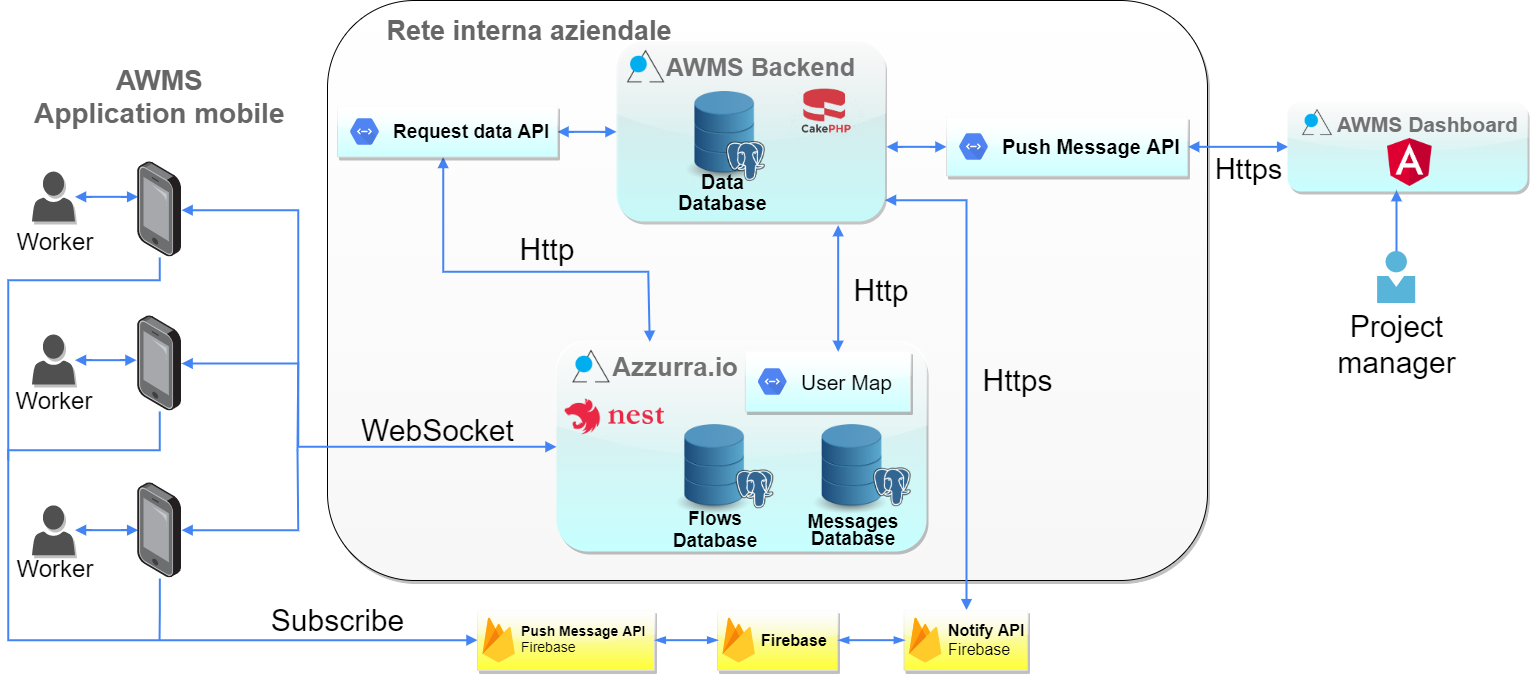
\includegraphics[scale=0.28]{AWMSDiagram.png}
 		\caption{Architettura di sistema AWMS}\label{fig:arch}
 	\end{center}
 \end{figure}
La figura precedente illustra come è composta l'\gls{architettura}\ap{[g]}, dove ogni componente verrà descritta nelle successive sotto sezioni.
\begin{trivlist}
	\item \subsection{AWMS Dashboard}
	È il pannello di controllo attraverso il quale un \gls{plant manager}\ap{[g]} interagisce con la piattaforma \gls{AWMS} per pianificare il lavoro da svolgere, cioè assegnare un compito alla persona più idonea. Il pannello di controllo è una applicazione web che è stata sviluppata in attraverso il \gls{framework}\ap{[g]} Angular.
	\begin{figure}[h] 
		\begin{center}
			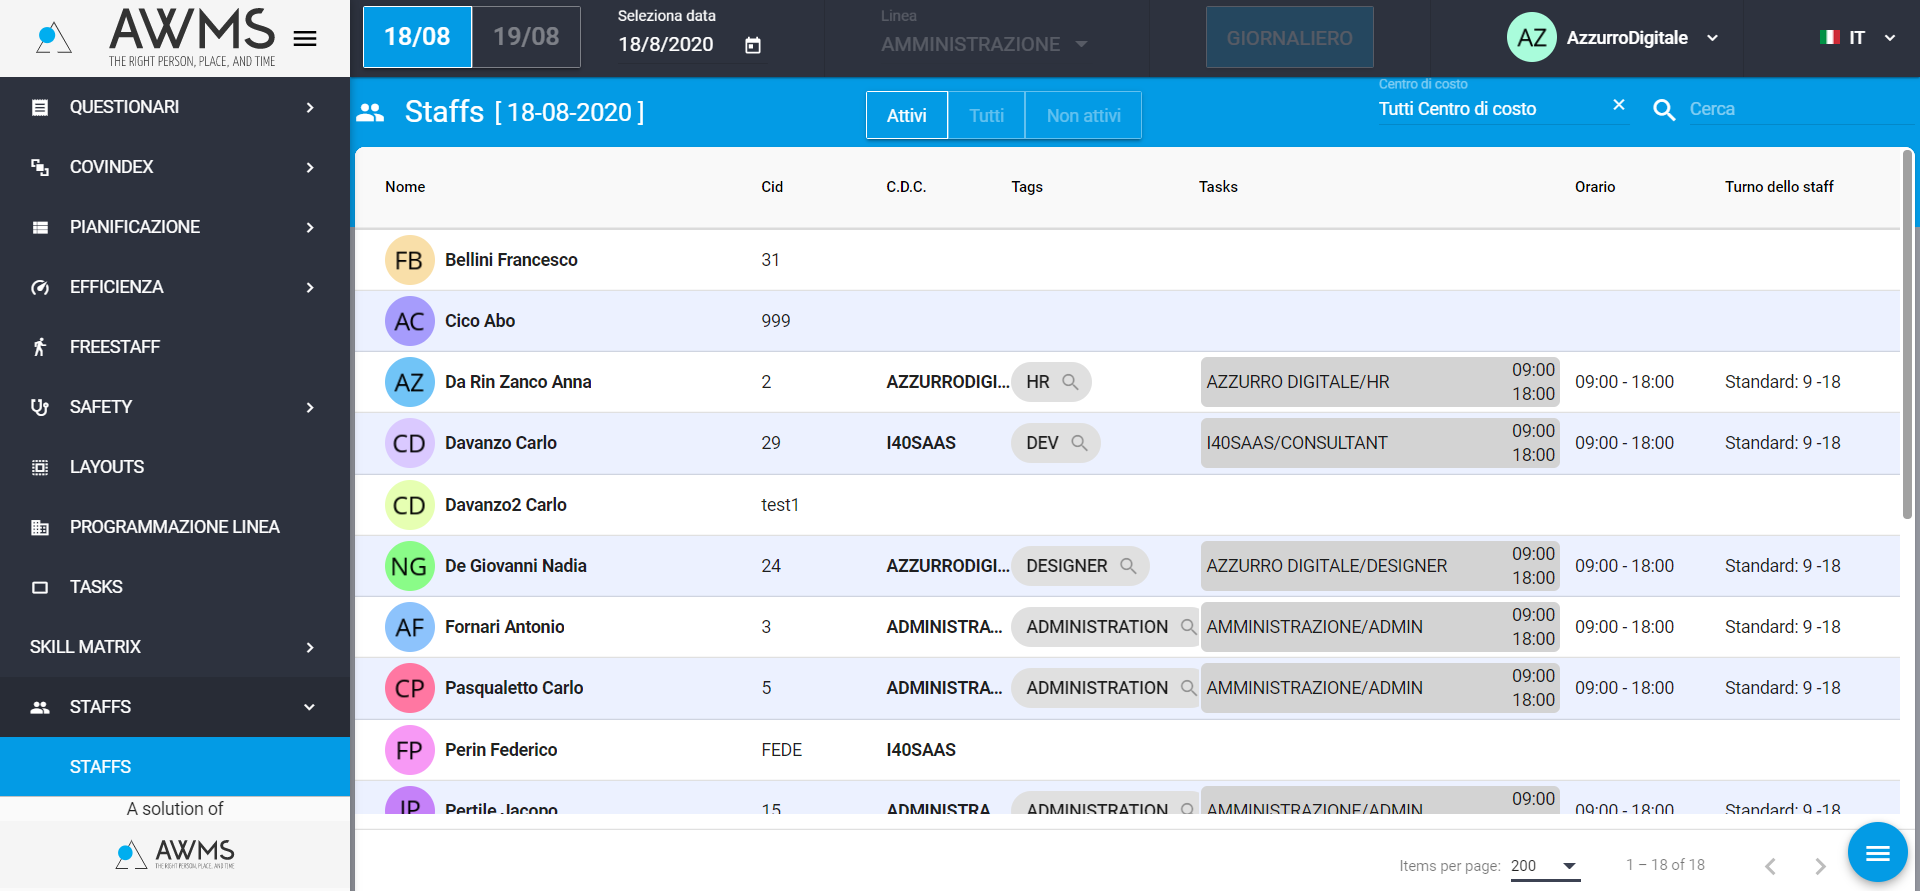
\includegraphics[height=8cm,width=13cm]{dashboardAWMS.png}
			\caption{Schermata di AWMS Dashboard}
		\end{center}
	\end{figure}
	 	La \emph{dashboard} per comunicare con il \gls{back-end}\ap{[g]}, utilizza delle \gls{api}\ap{[g]} che il back-end espone, quindi per una ragione di sicurezza, back-end e l'applicazione web cioè il front-end, comunicano attraverso \gls{api}\ap{[g]} con in più l'utilizzo del protocollo di comunicazione \gls{https}\glsfirstoccur che cripta la comunicazione. Nella Figura~\ref{fig:arch} viene mostrato il caso in cui il front-end utilizza \gls{api}\ap{[g]} per l'invio di una \gls{notifica push}\ap{[g]}, questo perché è previsto che quando il \gls{plant manager}\ap{[g]} sceglie il lavoratore più idoneo per un certo lavoro, quest'ultimo deve essere avvisato. Perciò sarà compito del front-end avvisare il back-end che c'è stata una nuova assegnazione e che questa assegnazione deve essere comunicata al diretto interessato attraverso un notifica sull'applicazione \emph{mobile} con all'interno Azzurra.
	\item \subsection{AWMS backend}
	Come dice il suo nome, AWMS Backend rappresenta il back-end del sistema. AWMS Backend è stato sviluppato usando la tecnologia CakePHP, un \gls{framework}\ap{[g]} per lo sviluppo di applicazioni web scritto in PHP. Al suo interno risiede il \gls{database}\ap{[g]} che contiene tutte le informazioni sui lavoratori e tra questi quindi, i dati da mostrare nei messaggi di Azzurra come ad esempio il piano di lavoro che ha il lavoratore in uno specifico giorno, qualora ne venga fatta richiesta. Il database utilizza come \gls{DBMS}\glsfirstoccur PostgreSQL. \\
	
	Come scritto nel punto precedente, per comunicare con lui, espone delle \gls{api}\ap{[g]} per la comunicazione infatti, esiste un \gls{api}\ap{[g]} per l'invio di una \gls{notifica push}\ap{[g]} ma esiste anche un \gls{api}\ap{[g]}, utilizzata da Azzurra.io, per la richiesta di informazioni sul lavoratore necessarie per completare il flusso di conversazione. Quindi questa \gls{api}\ap{[g]} permetterà di richiedere dati al back-end che li cercherà nel suo database interno. Se l'interrogazione al database da esito positivo, ritornerà le informazioni richieste a Azzurra.io. Il back-end si trova all'interno della rete interna dell'azienda che ha acquistato la soluzione di AzzurroDigitale, anche Azzurra.io è all'interno della rete, perciò tra queste due componenti avviene attraverso il protocollo di comunicazione \gls{http}\ap{[g]}\glsfirstoccur. Il back-end ha la possibilità di comunicare direttamente con Azzurra.io quando deve inviare una \gls{notifica push}\ap{[g]} e ha necessità di sapere quali utenti sono attivi, cioè hanno una connessione aperta con Azzurra.io. Per gli utenti invece che non hanno una connessione aperte con Azzurra.io e quindi non sono attivi l'invio della notifica verrà fatto utilizzando i servizi offerti da Firebase, la cui comunicazione tra back-end e Firebase avviene tramite HTTPS perché Firebase è un servizio esterno.\\
	
	La gestione dell'invio di una \gls{notifica push}\ap{[g]} verrà comunque trattato in modo più dettagliato più avanti nel seguente capitolo.
	\item \subsection{Azzurra.io}
	Azzurra.io è una componente strategica per il funzionamento del \gls{bot}\ap{[g]} Azzurra. Azzurra.io è sviluppata attraverso il \gls{framework}\ap{[g]} NestJS. Al suo interno ha due database con \gls{DBMS}\ap{[g]} PostgreSQL. Il primo database contiene i flussi di conversazione che indicano al \gls{bot}\ap{[g]} la sequenza di passi che deve seguire durante la conversazione con l'utente umano, la struttura dei flussi conversazionali verrà spiegata in modo dettagliato al capitolo successivo. Il secondo database permette di memorizzare i messaggi fatti tra il \gls{bot}\ap{[g]} Azzurra e l'utente umano. La scelta di adottare quest'ultimo database è dettata dalle seguenti motivazioni:
	\begin{itemize}
		\item Per mantenere lo stato della conversazione cioè, se l'utente decide di non andare avanti con la conversazione e di continuarla in un secondo momento, grazie a questo database, in cui viene salvato lo stato della conversazione, l'utente potrà continuare la conversazione da dove l'aveva lasciata. Il mantenimento dello stato della conversazione non avviene per un tempo illimitato ma dura al massimo un'ora dopo di che lo stato verrà cancellato;
		\item Per una migliore \emph{user experience} si è scelto, nel caso in cui ci siano state delle conversazioni in precedenza, di mostrare i messaggi delle conversazioni precedenti, cosi che se l'utente ha bisogno di un’informazione che ha già chiesto precedentemente ma che si è dimenticato, basta che controlli i messaggi presenti nella \emph{chat} senza dover richiedere ad Azzurra l'informazione dimenticata.
	\end{itemize}
	La connessione tra l'applicazione mobile e Azzurra.io è possibile grazie ai \gls{WebSocket}\ap{[g]} che permettono di aprire una connessione tra i due e di mantenere sempre aggiornati i dati ad esempio, la struttura dei flussi di conversazione, qualora venissero aggiornati. Per tenere traccia degli utenti connessi con Azzurra.io tramite l'applicazione \emph{mobile}, viene utilizzata una mappa chiave-valore, interna ad Azzurra.io, denominata \emph{User Map}. Grazie a essa Azzurra.io potrà rispondere alle richieste del back-end quando avrà bisogno della lista di utenti attivi per l'invio della di una \gls{notifica push}\ap{[g]}. Come scritto all'inizio della sotto sezione, Azzurro.ia è un componente strategico principalmente per due motivi.
	\begin{itemize}
		\item Quando si vuole aggiungere un nuovo flusso conversazionale o modificare un flusso già esistente, se non esistesse Azzurra.io, questi sarebbero salvati nell'applicazione. Ciò comporterebbe la necessità di un aggiornamento dell'applicazione \emph{mobile} e quindi di effettuare una nuova pubblicazione nell'Play Store per i dispositivi \gls{Android}\ap{[g]} e nel Apple Store per i dispositivi \gls{iOS}\ap{[g]} ad ogni aggiunta o modifica dei flussi. Grazie all'esistenza di Azzurra.io ciò viene evitato perché esiste il database dedicato per la memorizzazione dei flussi conversazionali che permette di aggiungere un nuovo flusso, semplicemente inserendolo all'interno del database, analogamente, questo vale anche per la modifica di un flusso. Inoltre, grazie alla connessione tramite \gls{WebSocket}\ap{[g]} qualunque modifica o aggiunta viene subito recepita dell'applicazione \emph{mobile};
		\item Per evitare che vengano fatte un numero elevato di richieste al back-end si è deciso di distribuire le informazioni in diverse componenti della rete, infatti il \gls{bot}\ap{[g]} per sapere che flusso conversazionale deve seguire per genere i messaggi per la conversazione con l'utente umano, chiede a Azzurra.io e non al back-end. Il backend però verrà contattato quando il \gls{bot}\ap{[g]} Azzurra ha bisogno di dati sul lavoratore da mostrare, questa richiesta però sarà fatta inizialmente a Azzurra.io che si prenderà carico di richiedere le informazioni al backend e di ritornarle all'applicazione. Quindi il backend sarà contattato solo dalla \emph{dashboard} e da Azzurra.io per il caso descritto precedentemente o per il processo di autenticazione dell'utente, diminuendo il carico sul back-end.
	\end{itemize}
	
	\item\subsection{Applicazione mobile AWMS}
	L'ultimo componente dell'\gls{architettura}\ap{[g]} è l'applicazione \emph{mobile} \gls{AWMS}. Essa è sviluppata attraverso il \gls{framework}\ap{[g]} Angular2+ e Ionic. L'applicazione \emph{mobile} è in realtà un'\gls{applicazione ibrida}\ap{[g]}, questo perché viene sviluppata con tecnologie web, nello specifico \gls{HTML}, \gls{CSS} e TypeScript, e viene eseguita in un dispositivo \emph{mobile} grazie a Ionic e a Cordova. All'interno dell'applicazione \emph{mobile} risiede il \gls{bot}\ap{[g]} Azzurra. Oltre al \gls{bot}\ap{[g]} Azzurra esistono altre due sezioni, la sezione Questionario e la sezione Profilo. 
	
	\begin{figure}[h]
		\centering
		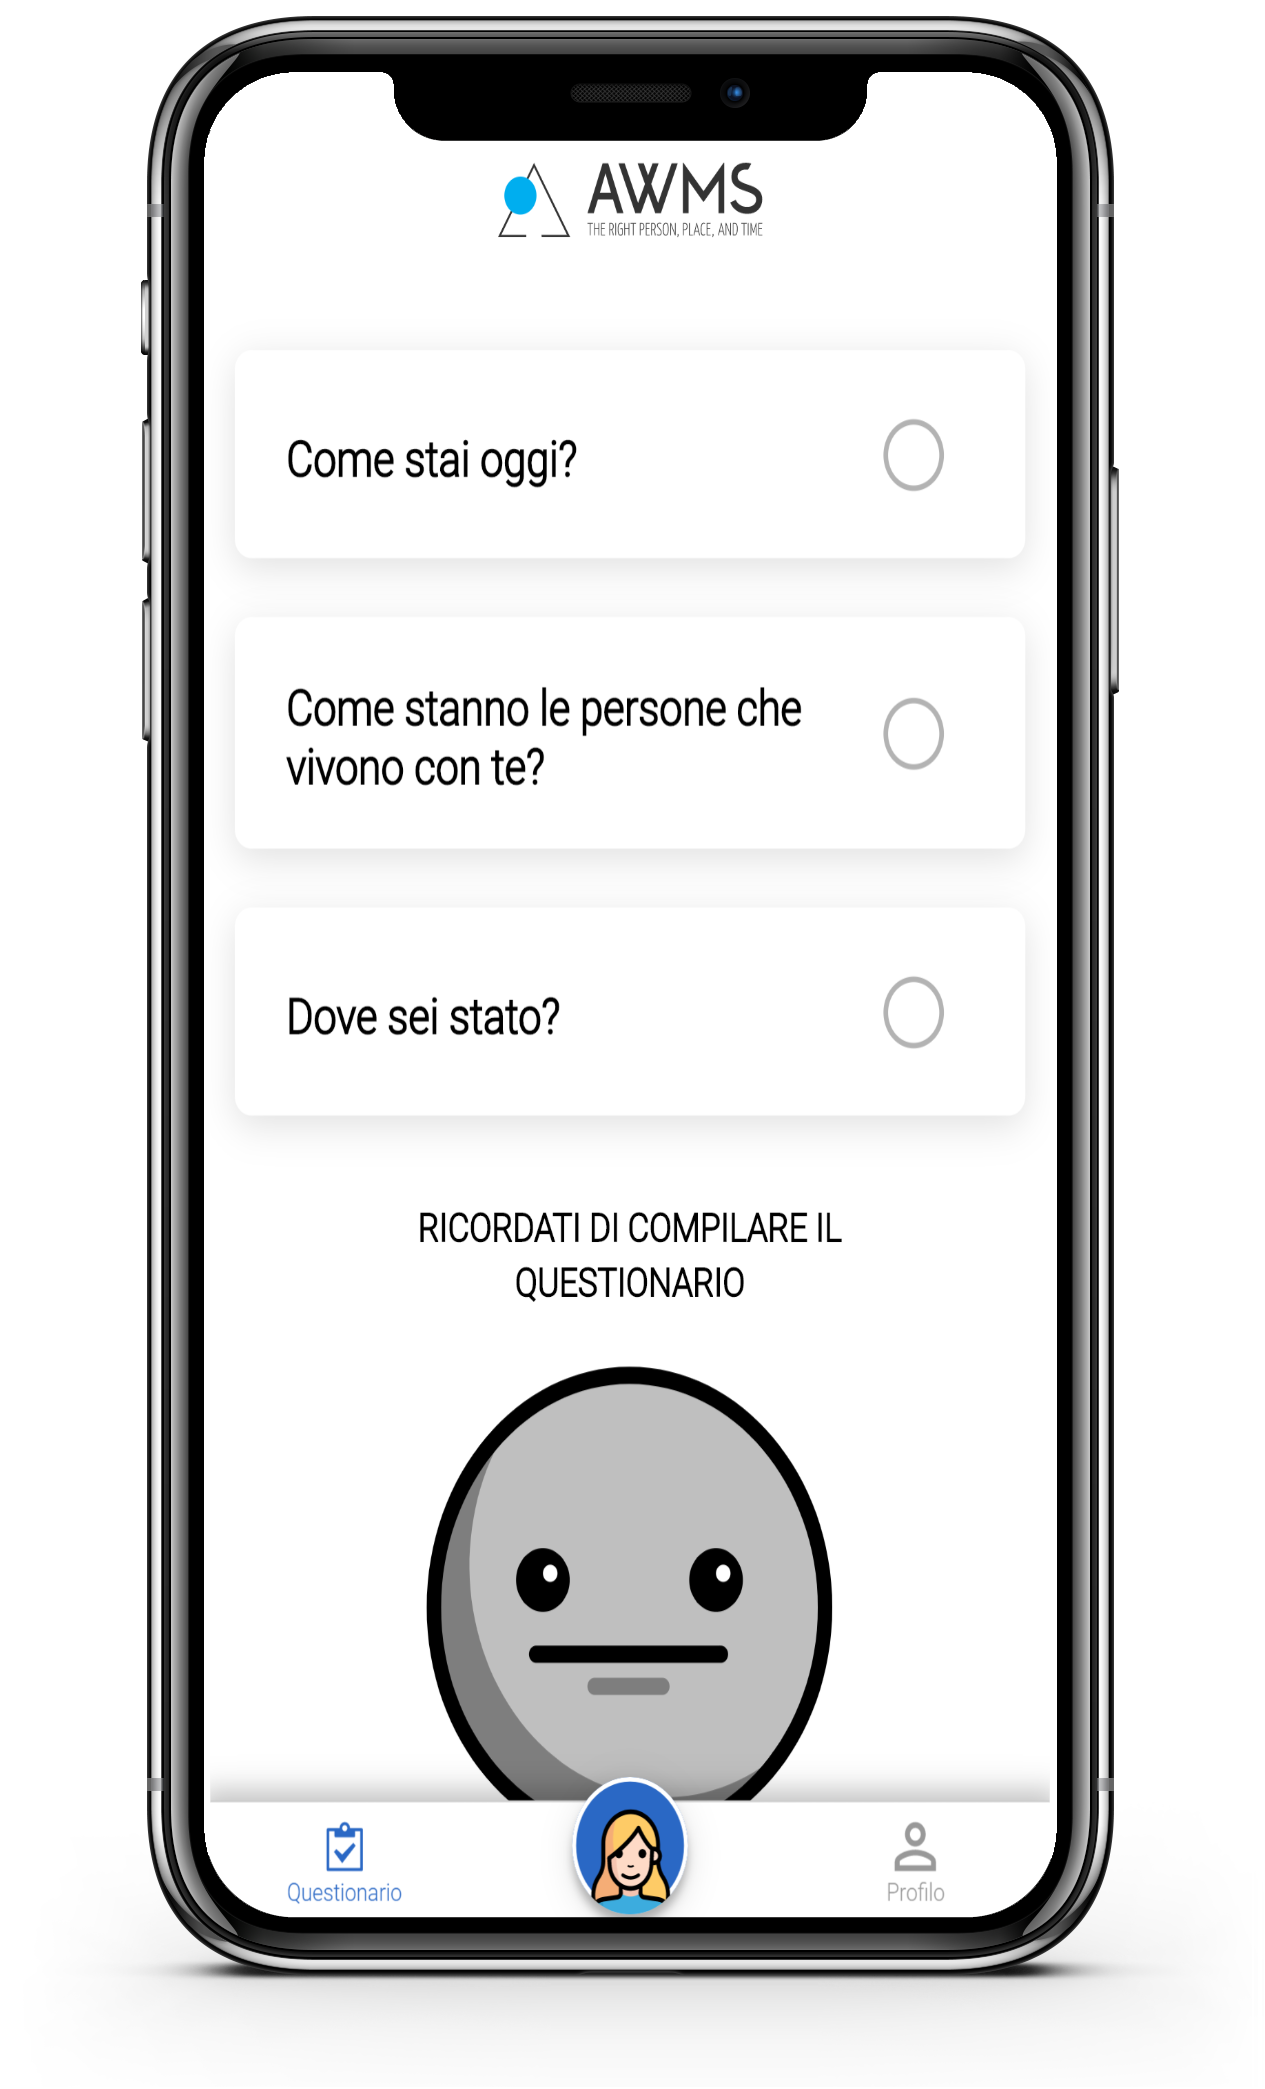
\includegraphics[scale=0.13]{queGrey.png}\hfill
		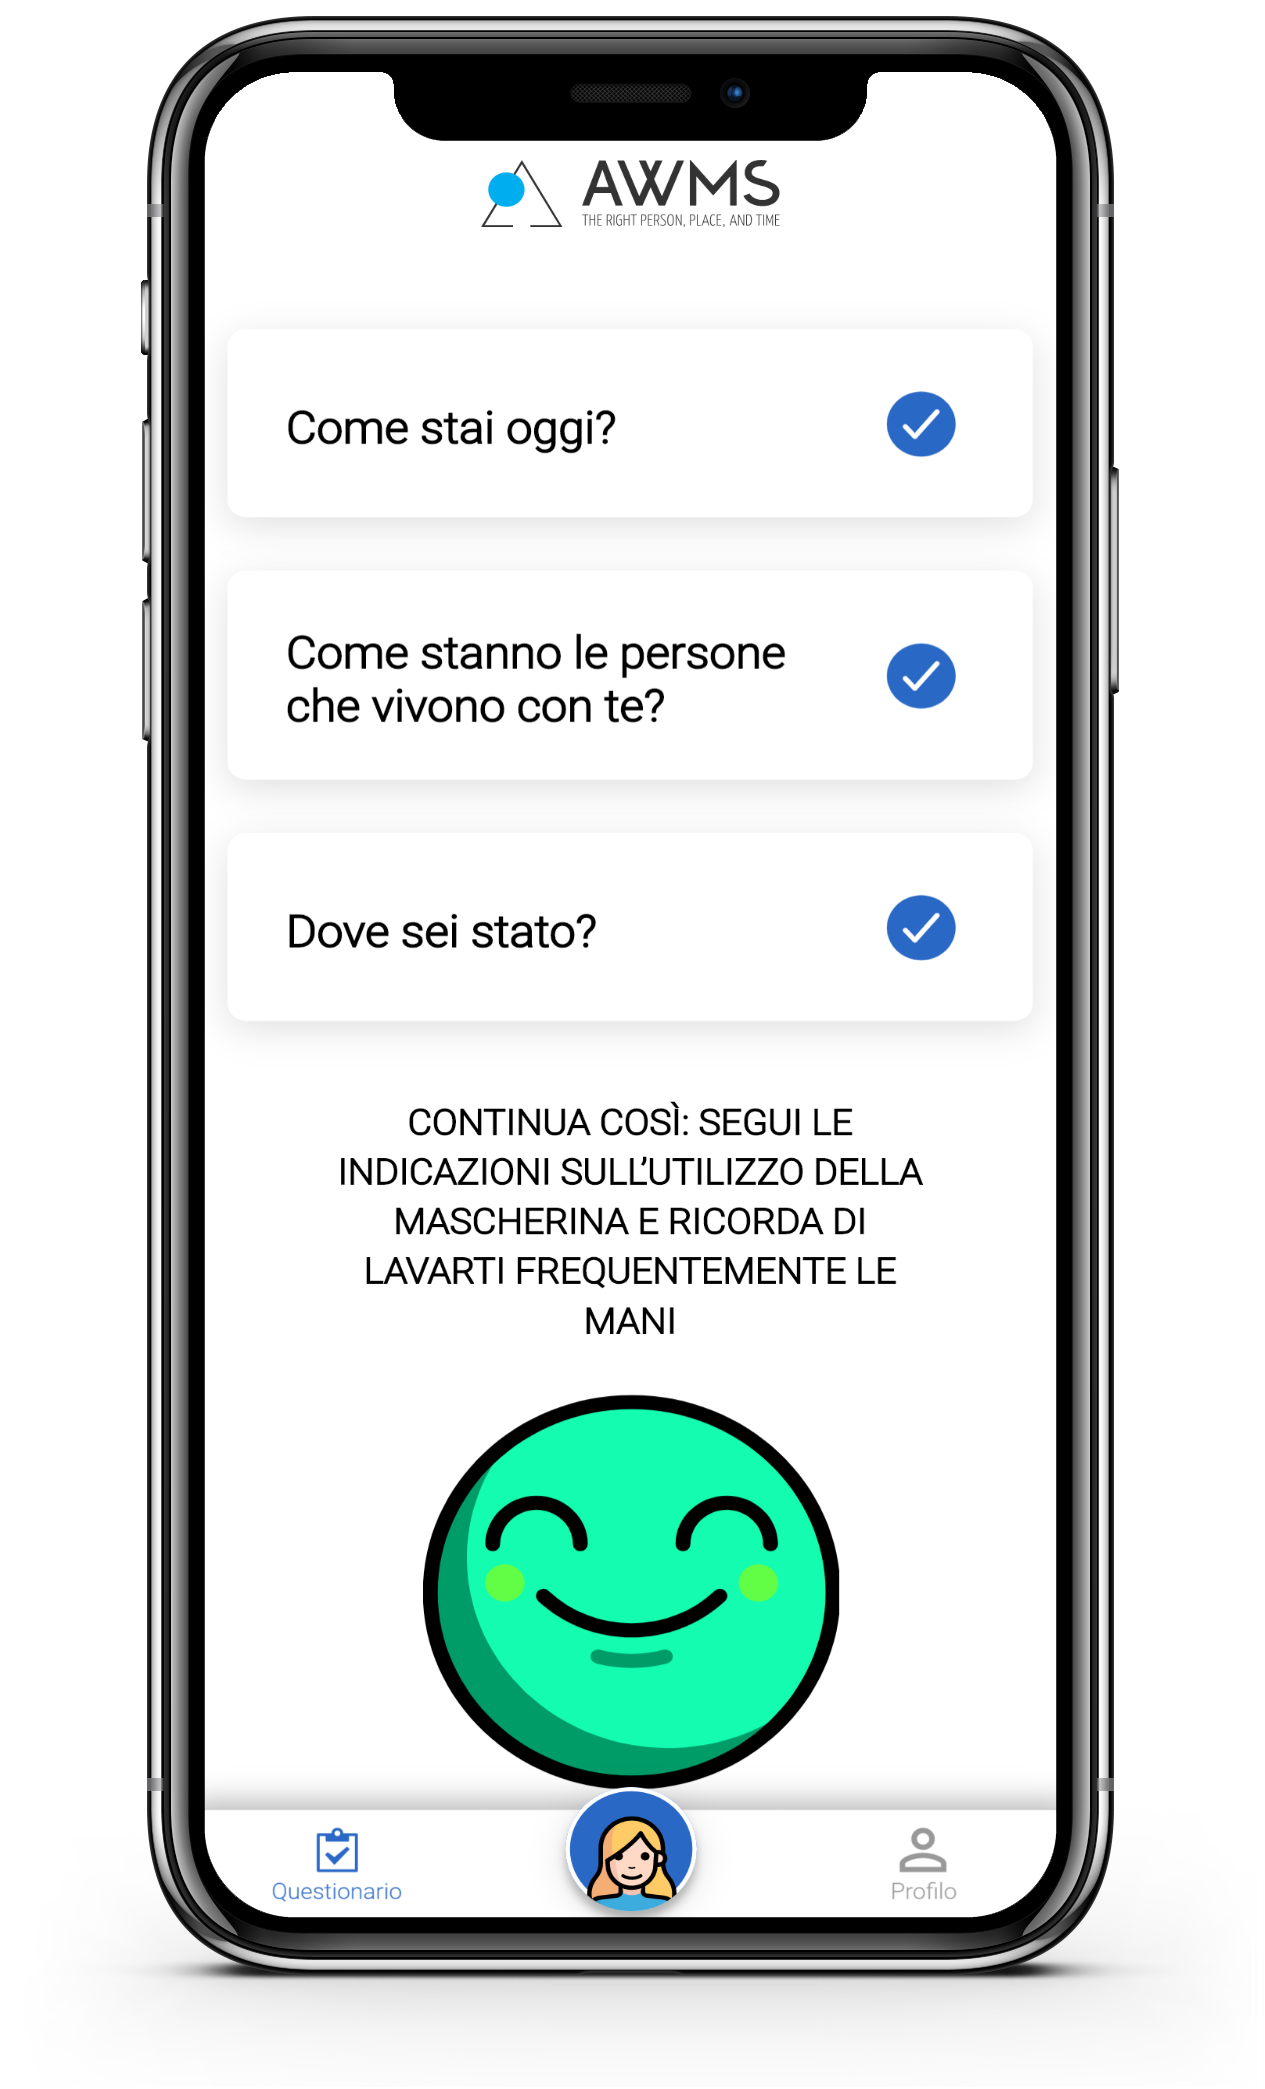
\includegraphics[scale=0.13]{queGreen.png}\hfill
		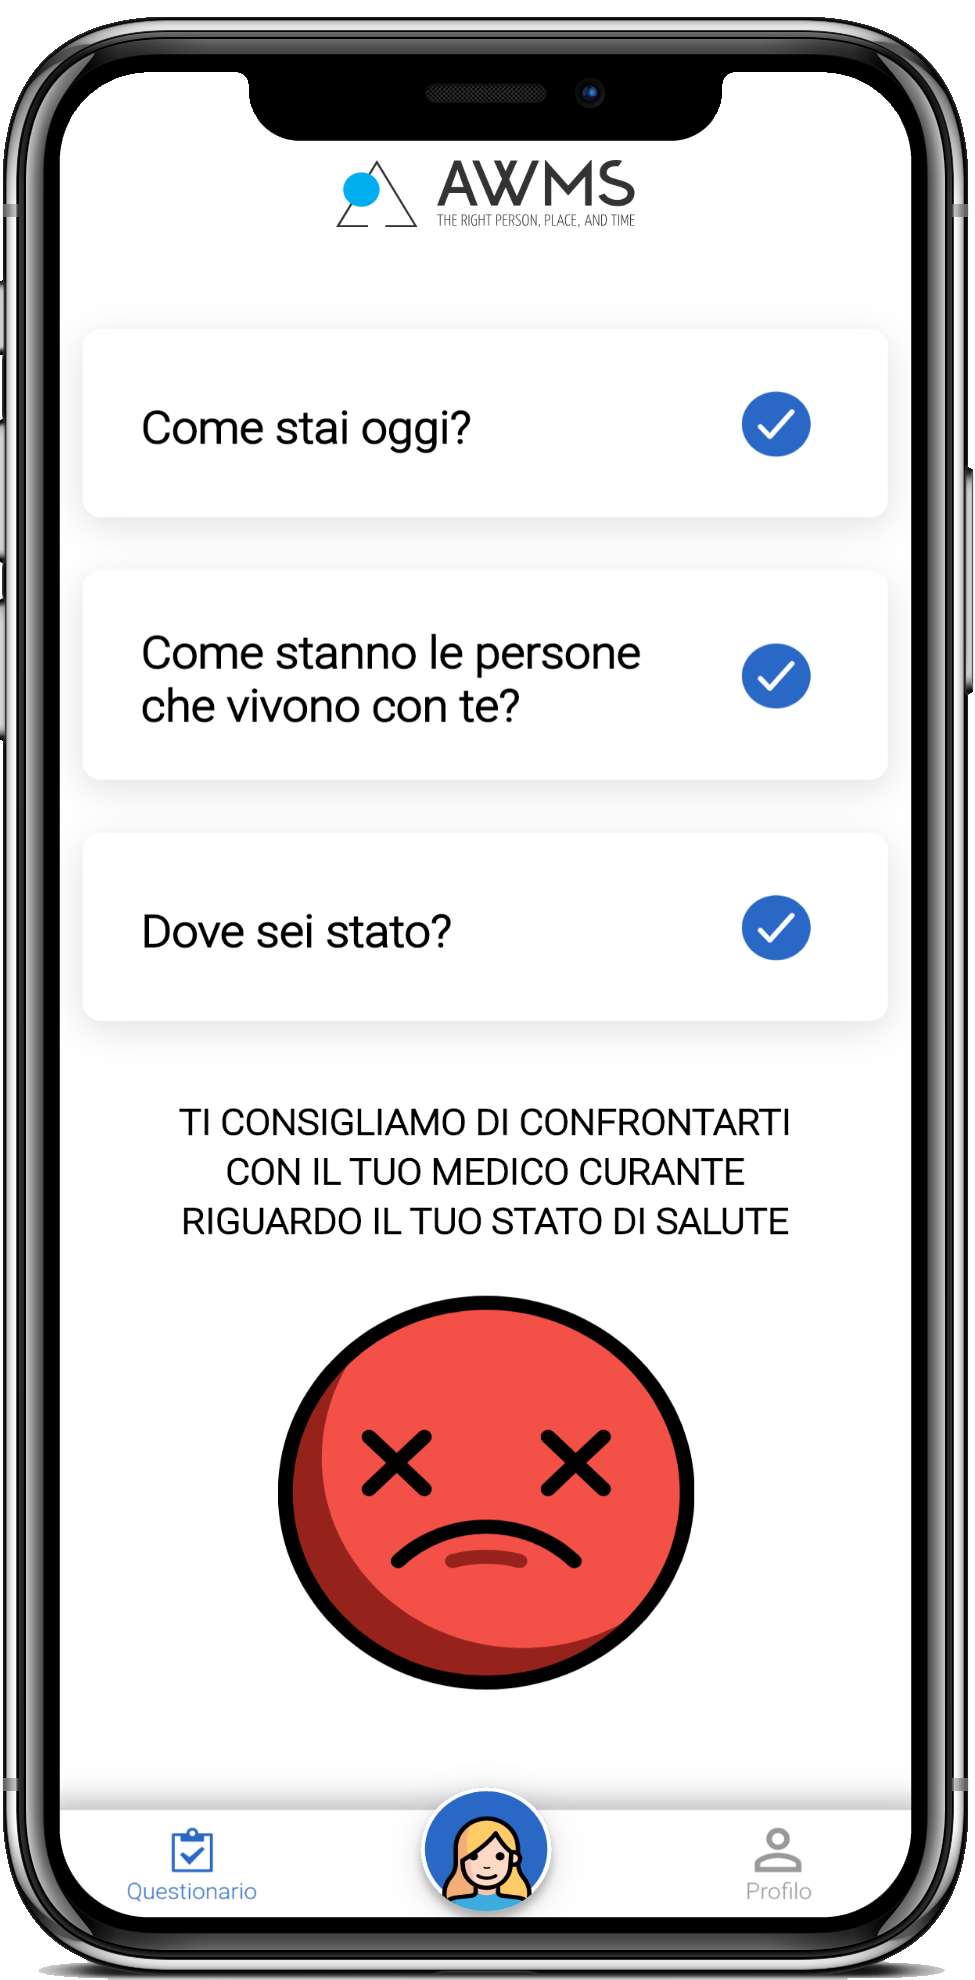
\includegraphics[scale=0.13]{queRed.png}
		\caption{Sezione Questionario}\label{fig:que}
	\end{figure}
	
	La Figura~\ref{fig:que} mostra la sezione Questionario nei suoi 3 possibili stati. In questa sezione viene richiesto di compilare quotidianamente un questionario in cui vengono poste domande sulla propria salute che, dai dati raccolti per ogni lavoratore l'applicazione cerca di capire se all'interno dell'azienda ci sia pericolo di contagio del virus COVID-19. Nel caso in cui non si è ancora compilato il questionario, viene mostrata una faccina grigia come si può vedere nella prima immagine della Figura~\ref{fig:que}. Se si è compilato il questionario e secondo le risposte date si risulta essere in buona salute, allora l'applicazione mostrerà una faccina verde come si può vedere nella seconda immagine della Figura~\ref{fig:que}. Se si è compilato il questionario e secondo le risposte date si risulta essere a rischio per la propria salute, allora l'applicazione mostrerà una faccina rossa come si può vedere dalla terza immagine della Figura~\ref{fig:que}.
	
	Nel questionario da compilare vengono richiesti se si hanno avuto dei sintomi di malattie come mostra la prima immagine della Figura~\ref{fig:queSlide}. Successivamente viene richiesto se le persone vicino a noi hanno avuto dei sintomi di malattie come mostrato nella seconda immagine della Figura~\ref{fig:queSlide}. Viene poi richiesto in quelli luoghi si è stati come mostrato nella terza immagine della Figura~\ref{fig:queSlide}.
	\begin{figure}[h]
		\begin{center}
			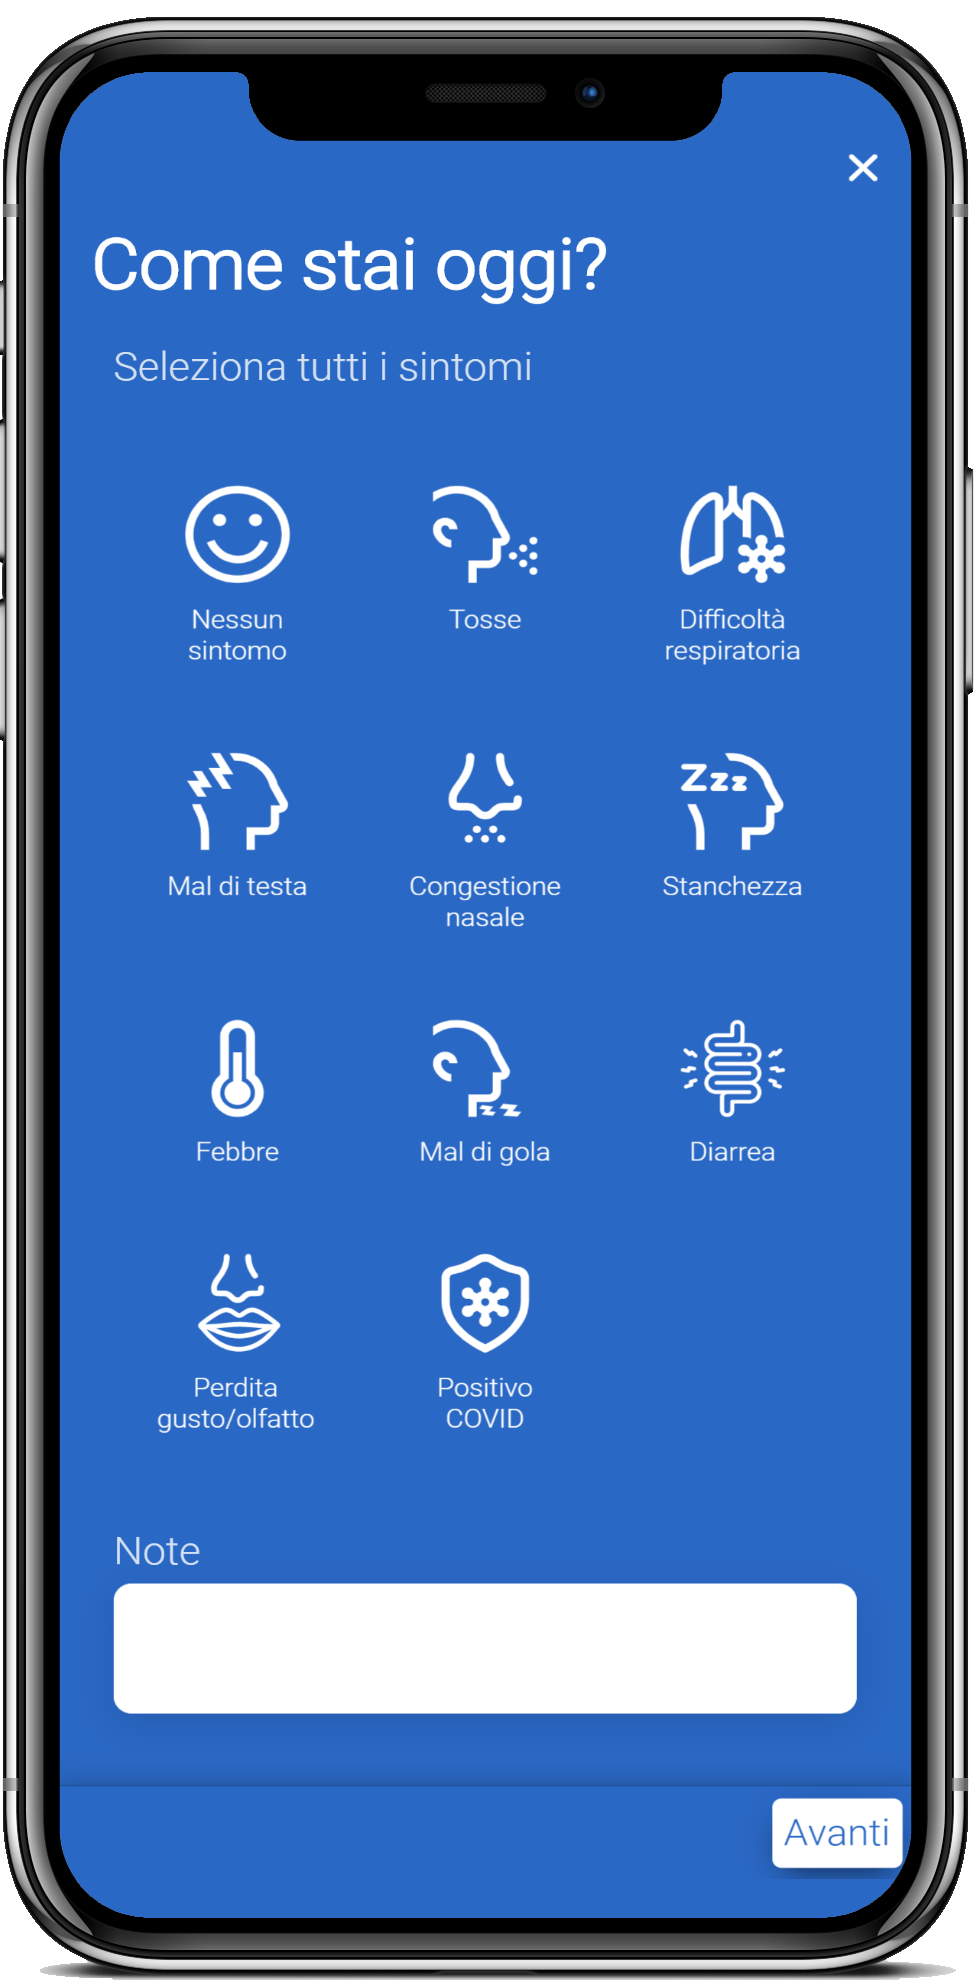
\includegraphics[scale=0.124]{que1.png}\hfill
			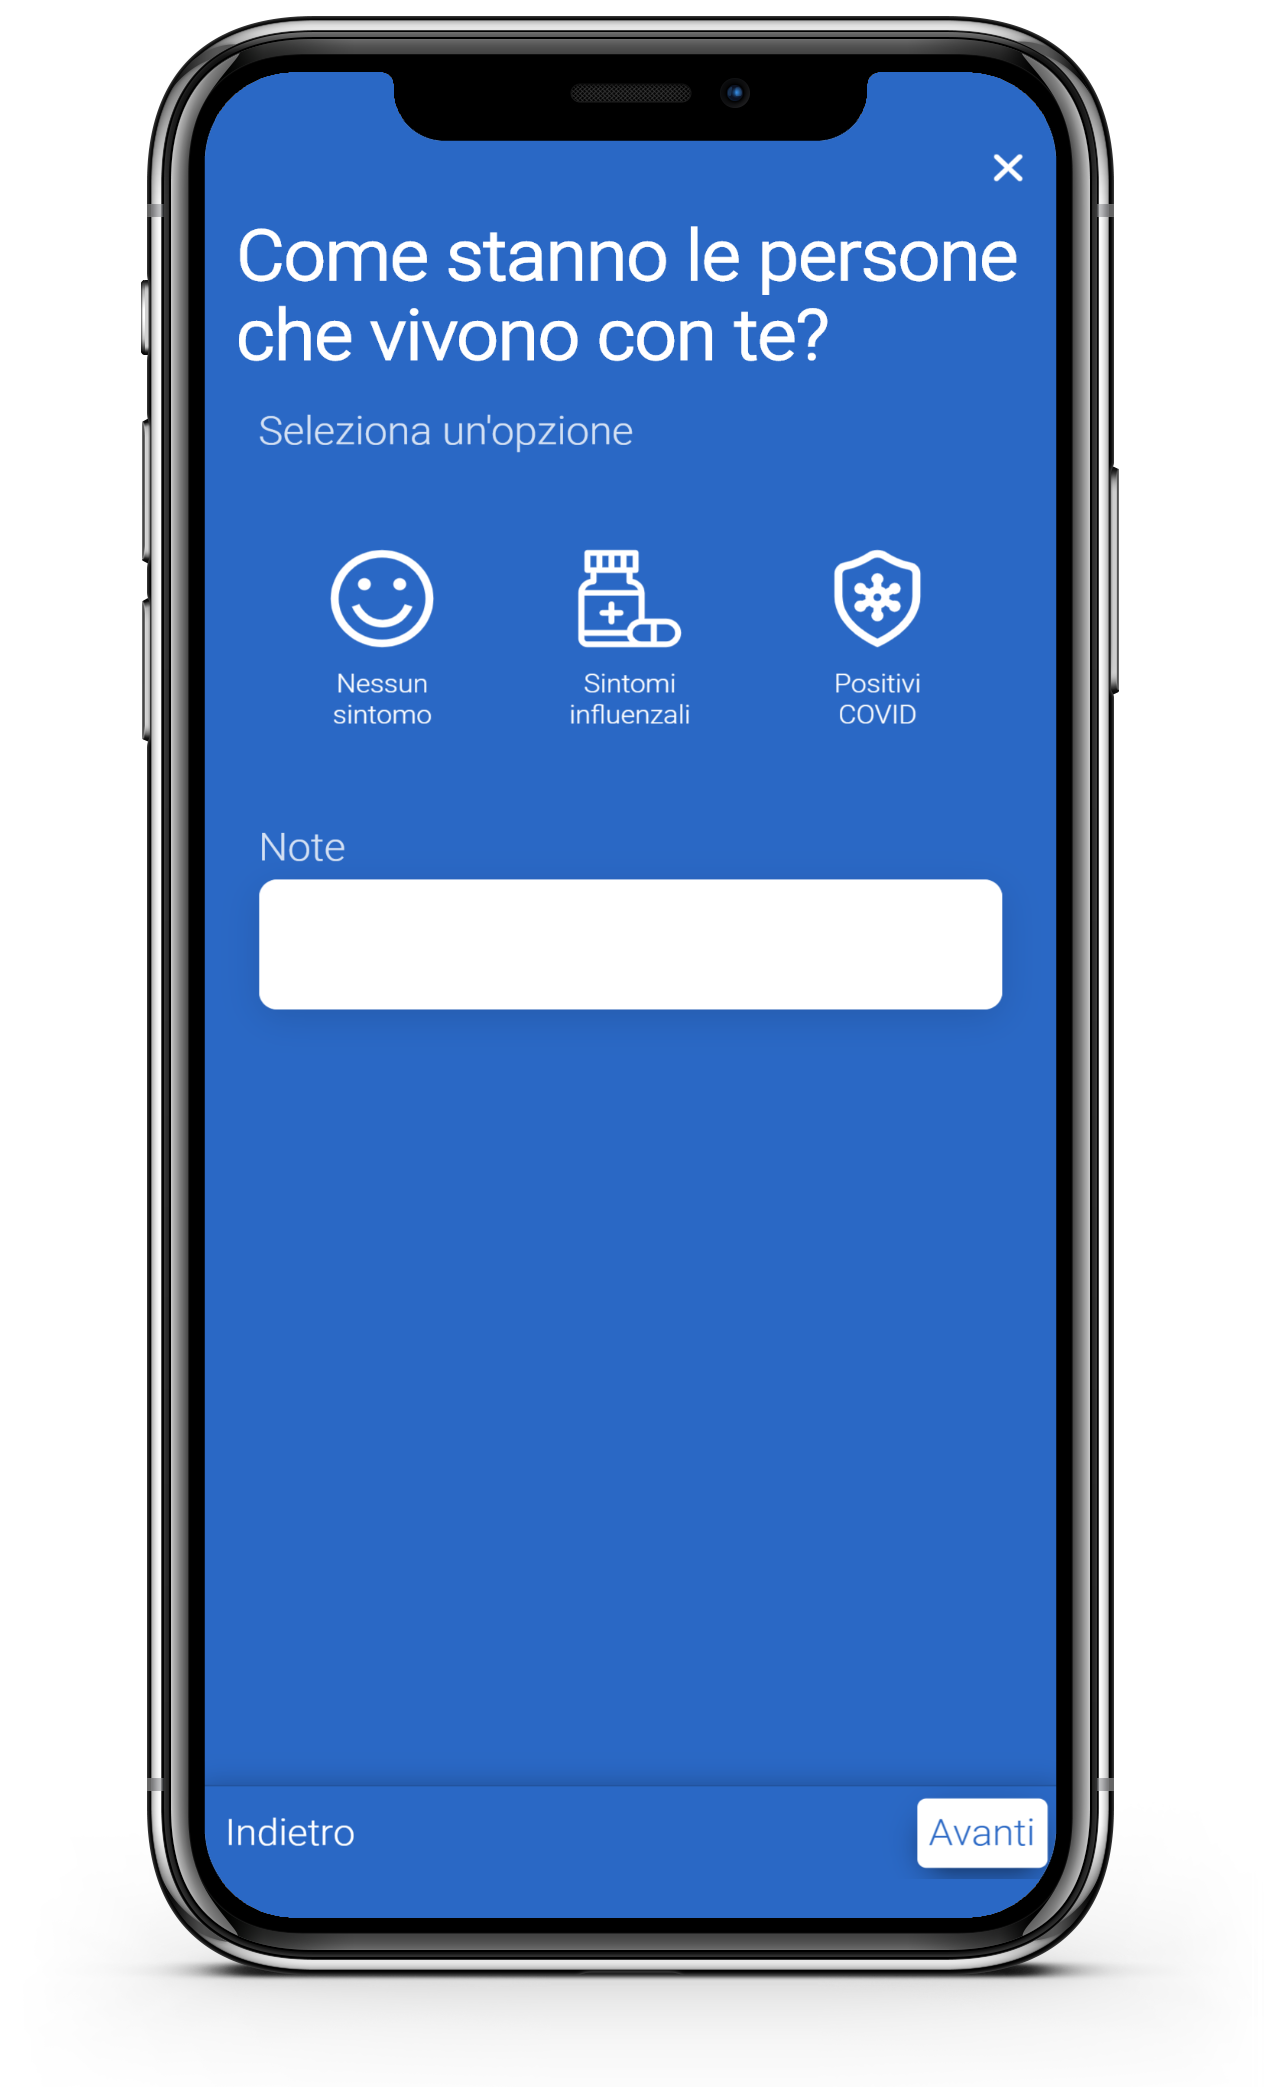
\includegraphics[scale=0.124]{que2.png}\hfill
			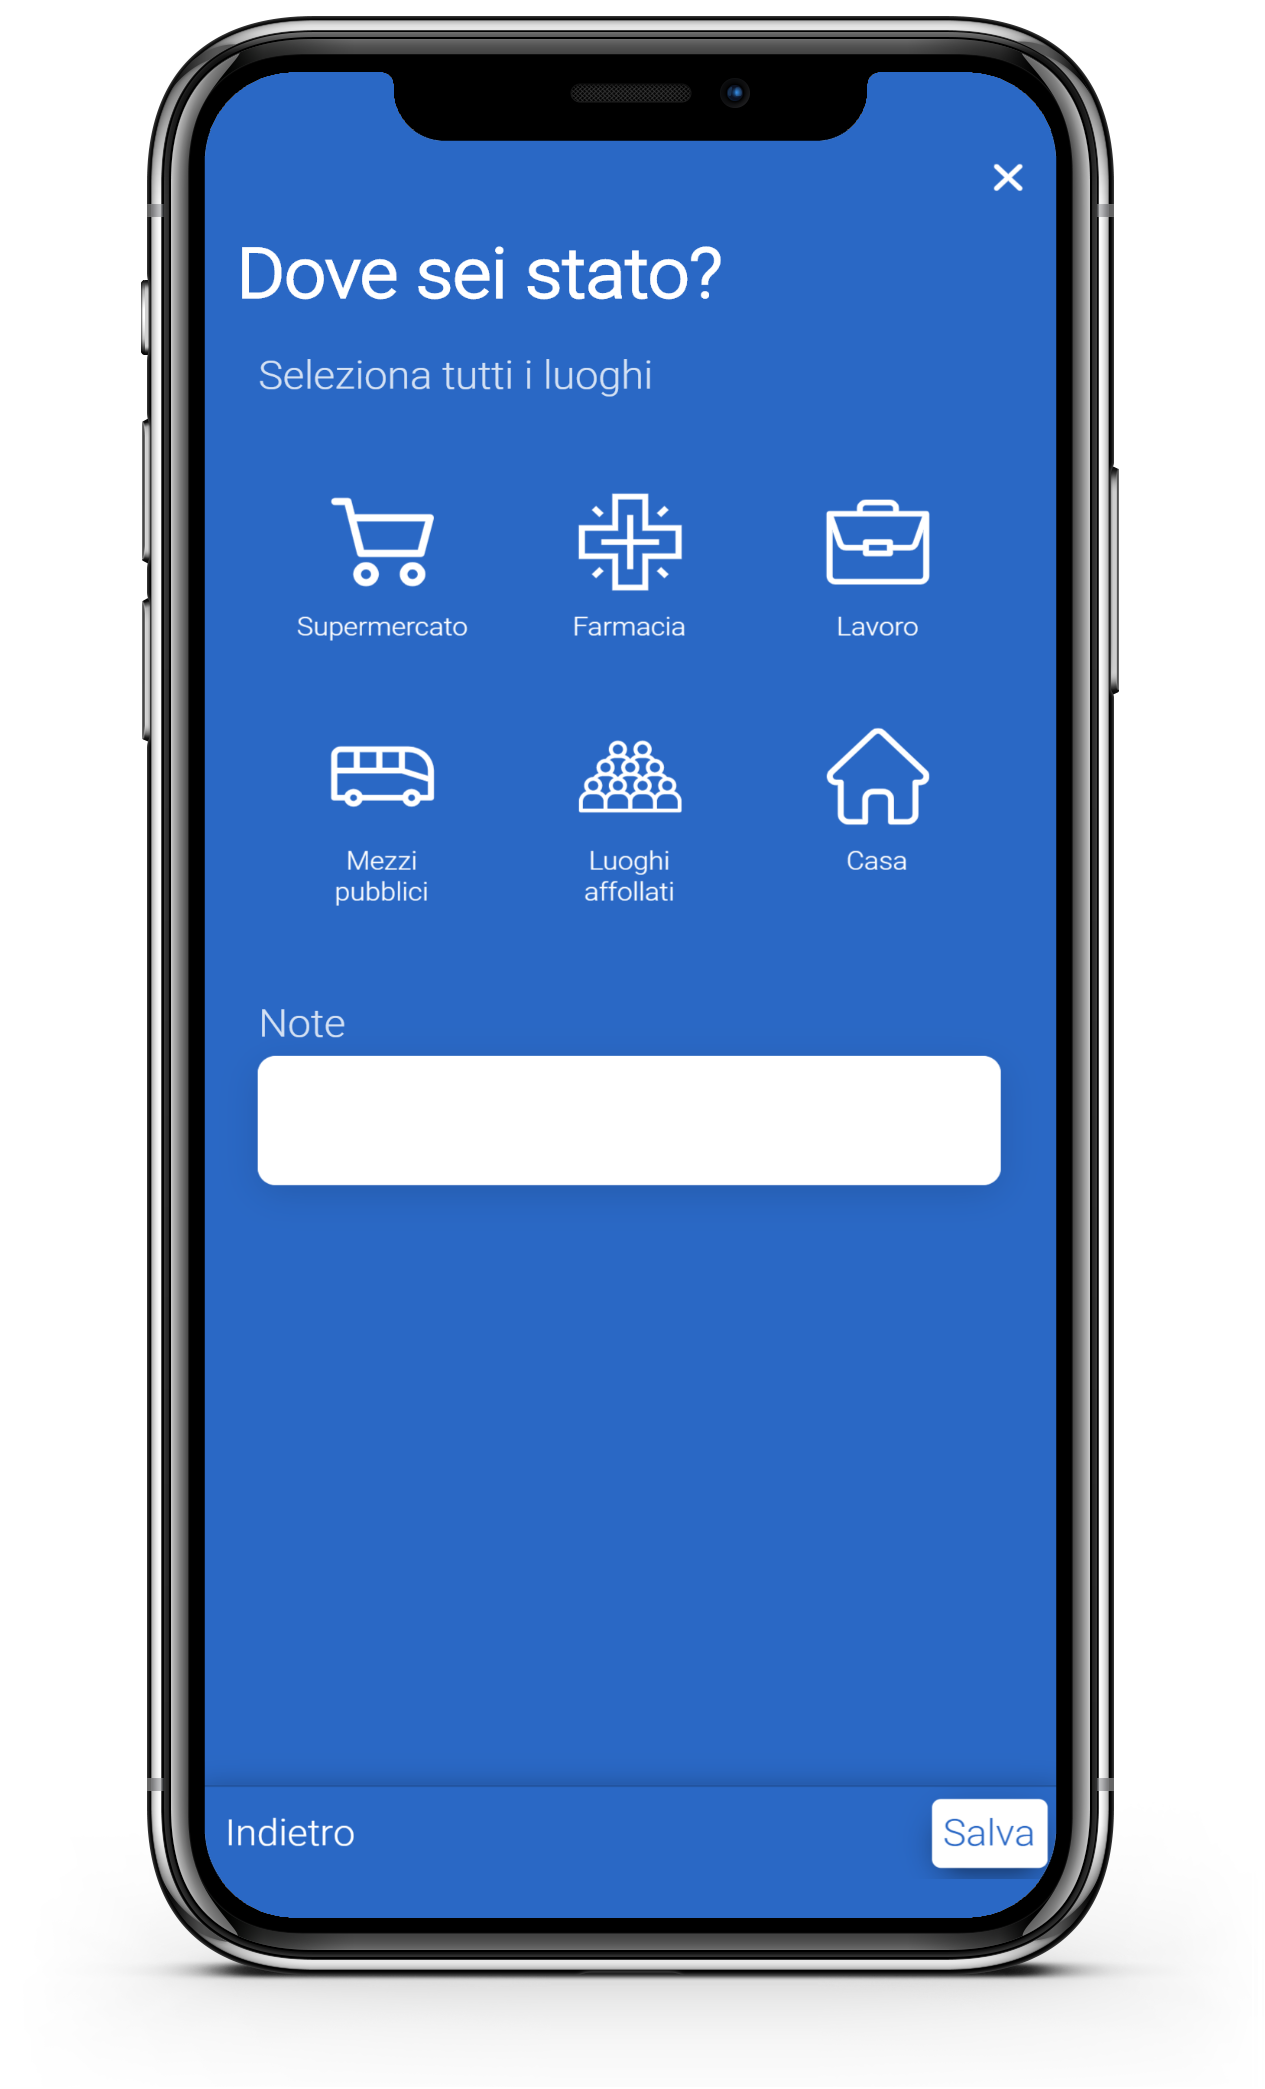
\includegraphics[scale=0.124]{que3.png}
			\caption{Schede del questionario sulla salute}\label{fig:queSlide}
		\end{center}
	\end{figure}
	Una volta terminato il questionario, l'applicazione elaborare le risposte date e mostrerà l'esito sulla nostra salute. Nel caso in cui l'esito sia positivo verrà mostrata la prima immagine della Figura~\ref{fig:quefinal} invece in caso di esito negativo verrà mostrata la seconda immagine della Figura~\ref{fig:quefinal}.
	\begin{figure}[h]
		\begin{center}
			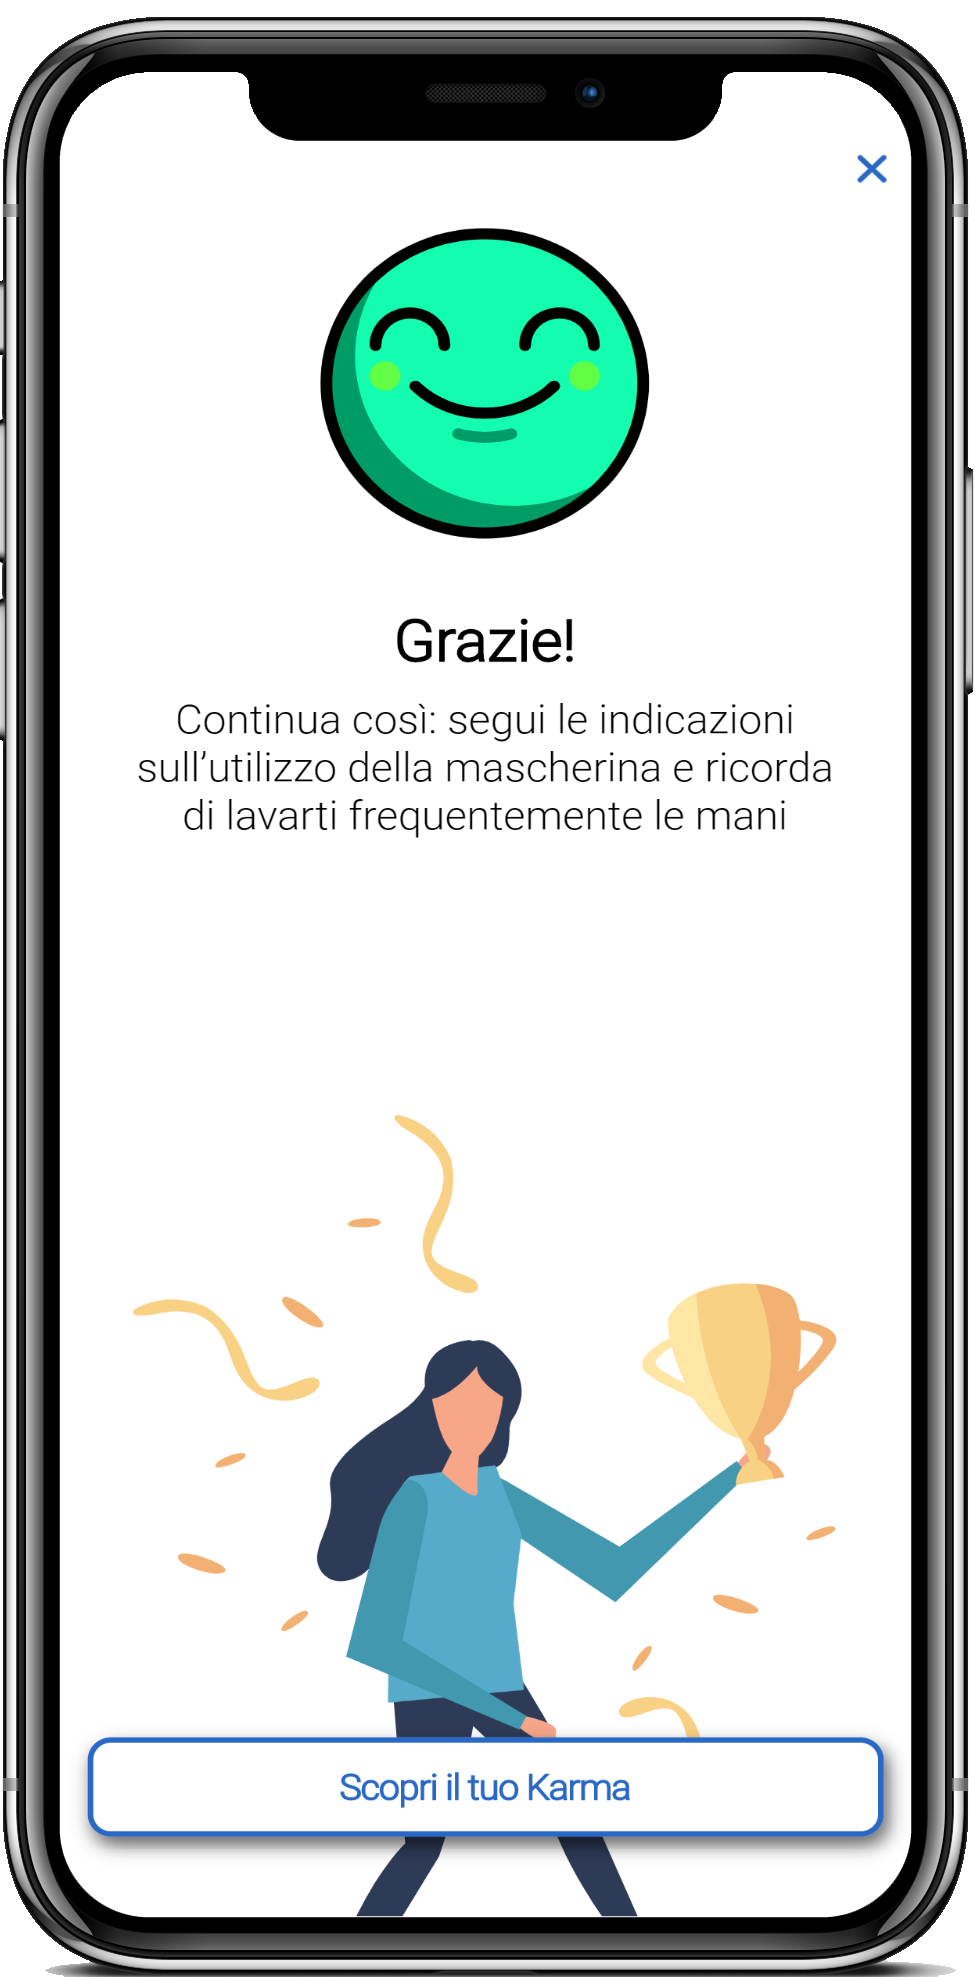
\includegraphics[scale=0.124]{finalGreen.png}\hfil
			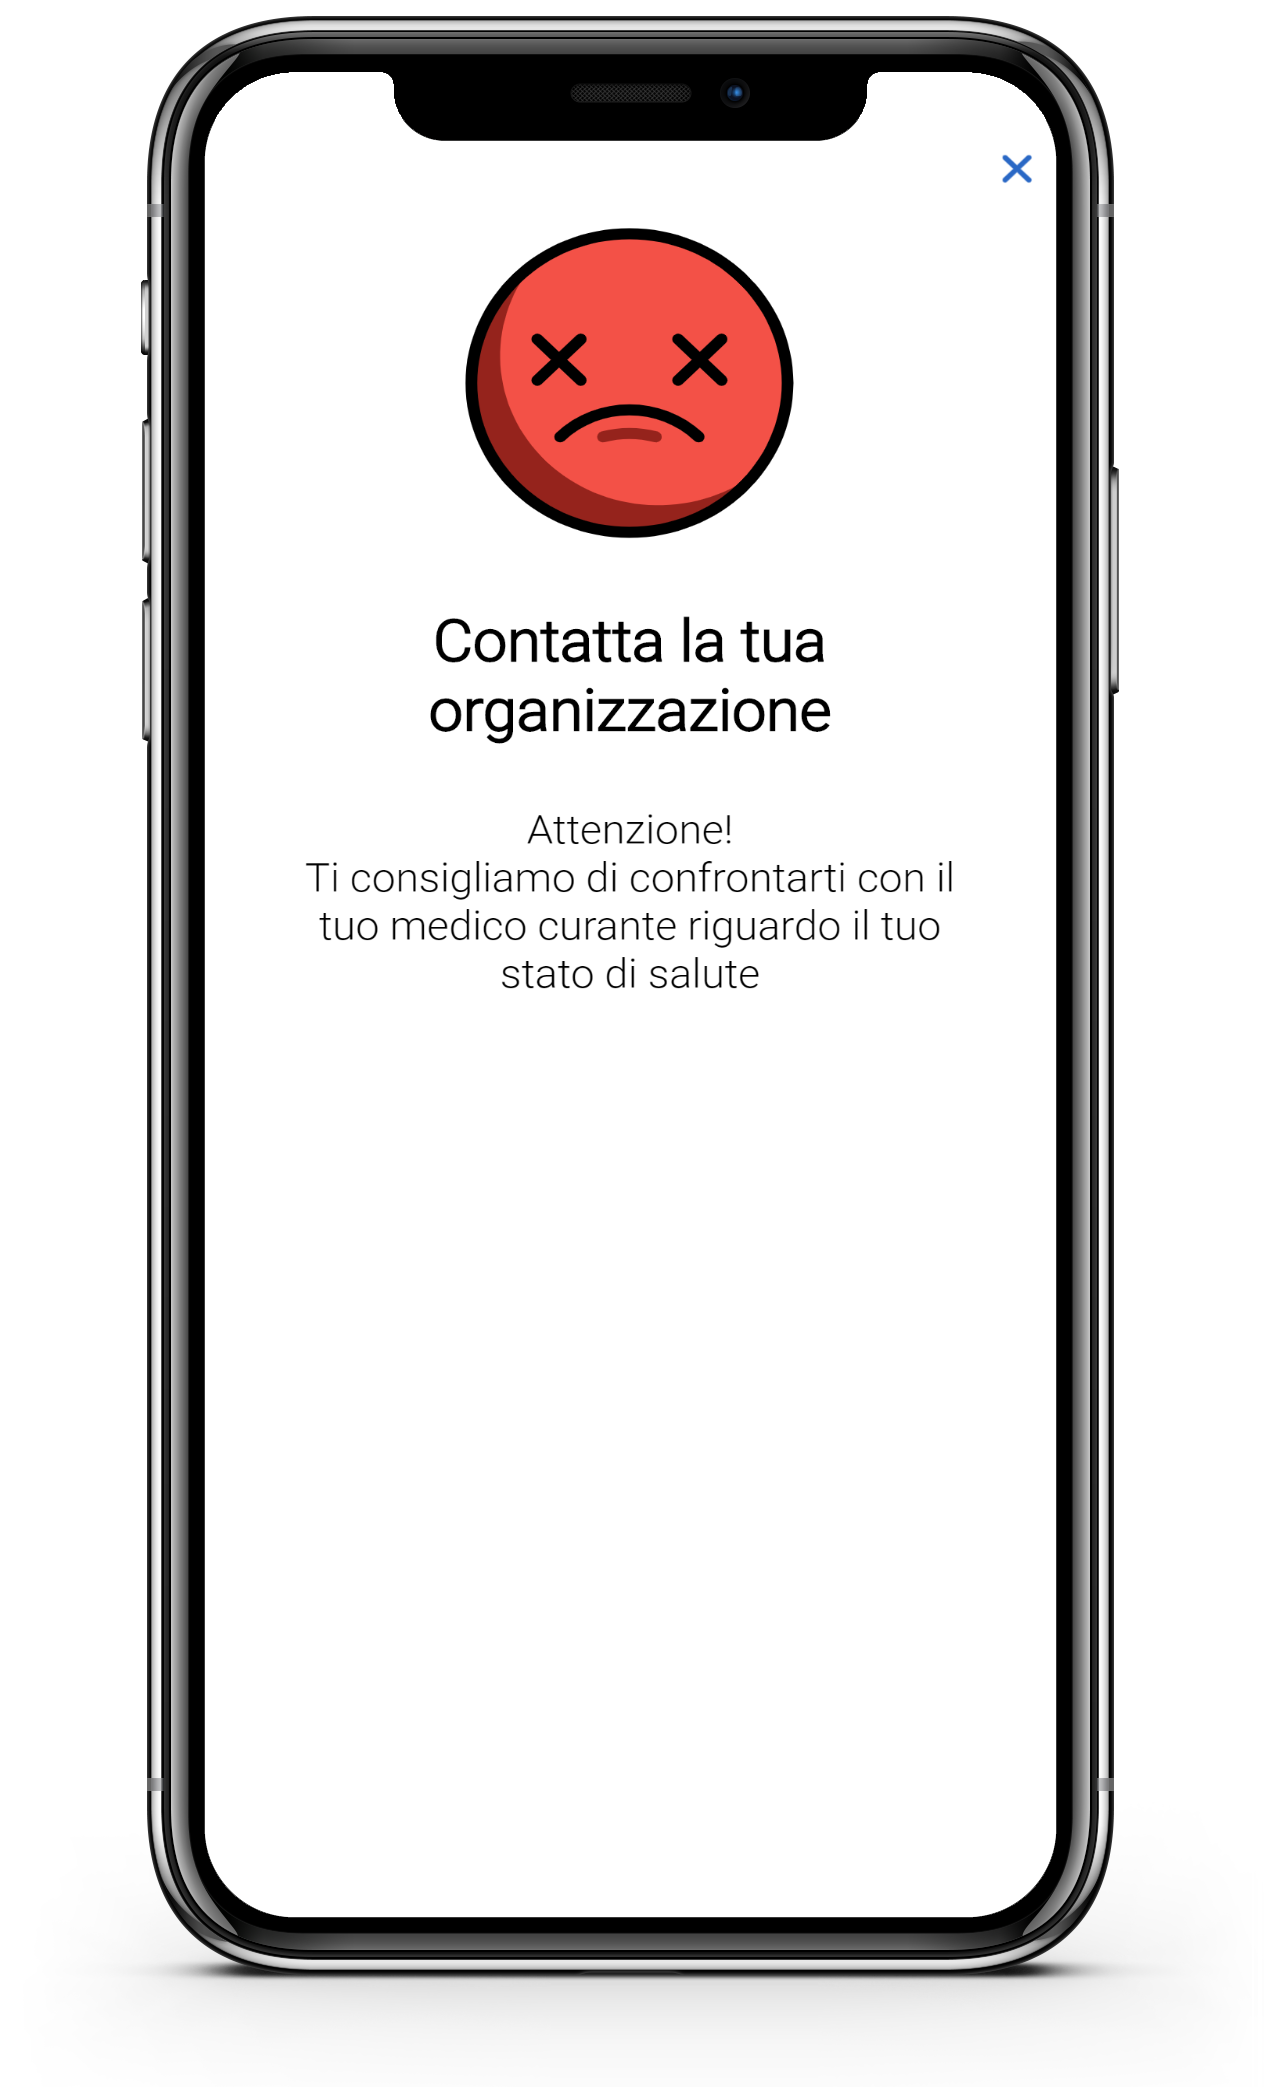
\includegraphics[scale=0.124]{finalRed.png}
			\caption{Schede dell'esito del questionario sulla salute}\label{fig:quefinal}
		\end{center}
	\end{figure}\\
	Il risultato viene poi riportato anche nella schermata della sezione Questionario.
	\\
	Nella sezione Profilo invece, vengono mostrati i Karma points che sono stati raccolti durante la compilazione del questionario, punti che al momento non danno nessun particolare beneficio ma, in futuro è previsto l'implementazione di una qualche ricompensa. Vengono mostrate le proprie informazioni personali cliccando il tasto "Informazioni personali" come mostrato in Figura~\ref{fig:profile}, è possibile cambiare la password d'accesso cliccando il bottone "Gestione password". Cliccando il bottone Istruzione di utilizzo mostrato sempre nella Figura~\ref{fig:profile} è possibile accedere a una breve guida su come utilizzare l'applicazione. Nel bottone "Normativa privacy" è possibile visionare la normativa sulla tutela della \emph{privacy} \gls{GDPR}\glsfirstoccur mentre nel bottone "Titolare trattamento" viene indicato da chi vengono trattati i dati inseriti.
	\begin{figure}[h]
		\begin{center}
			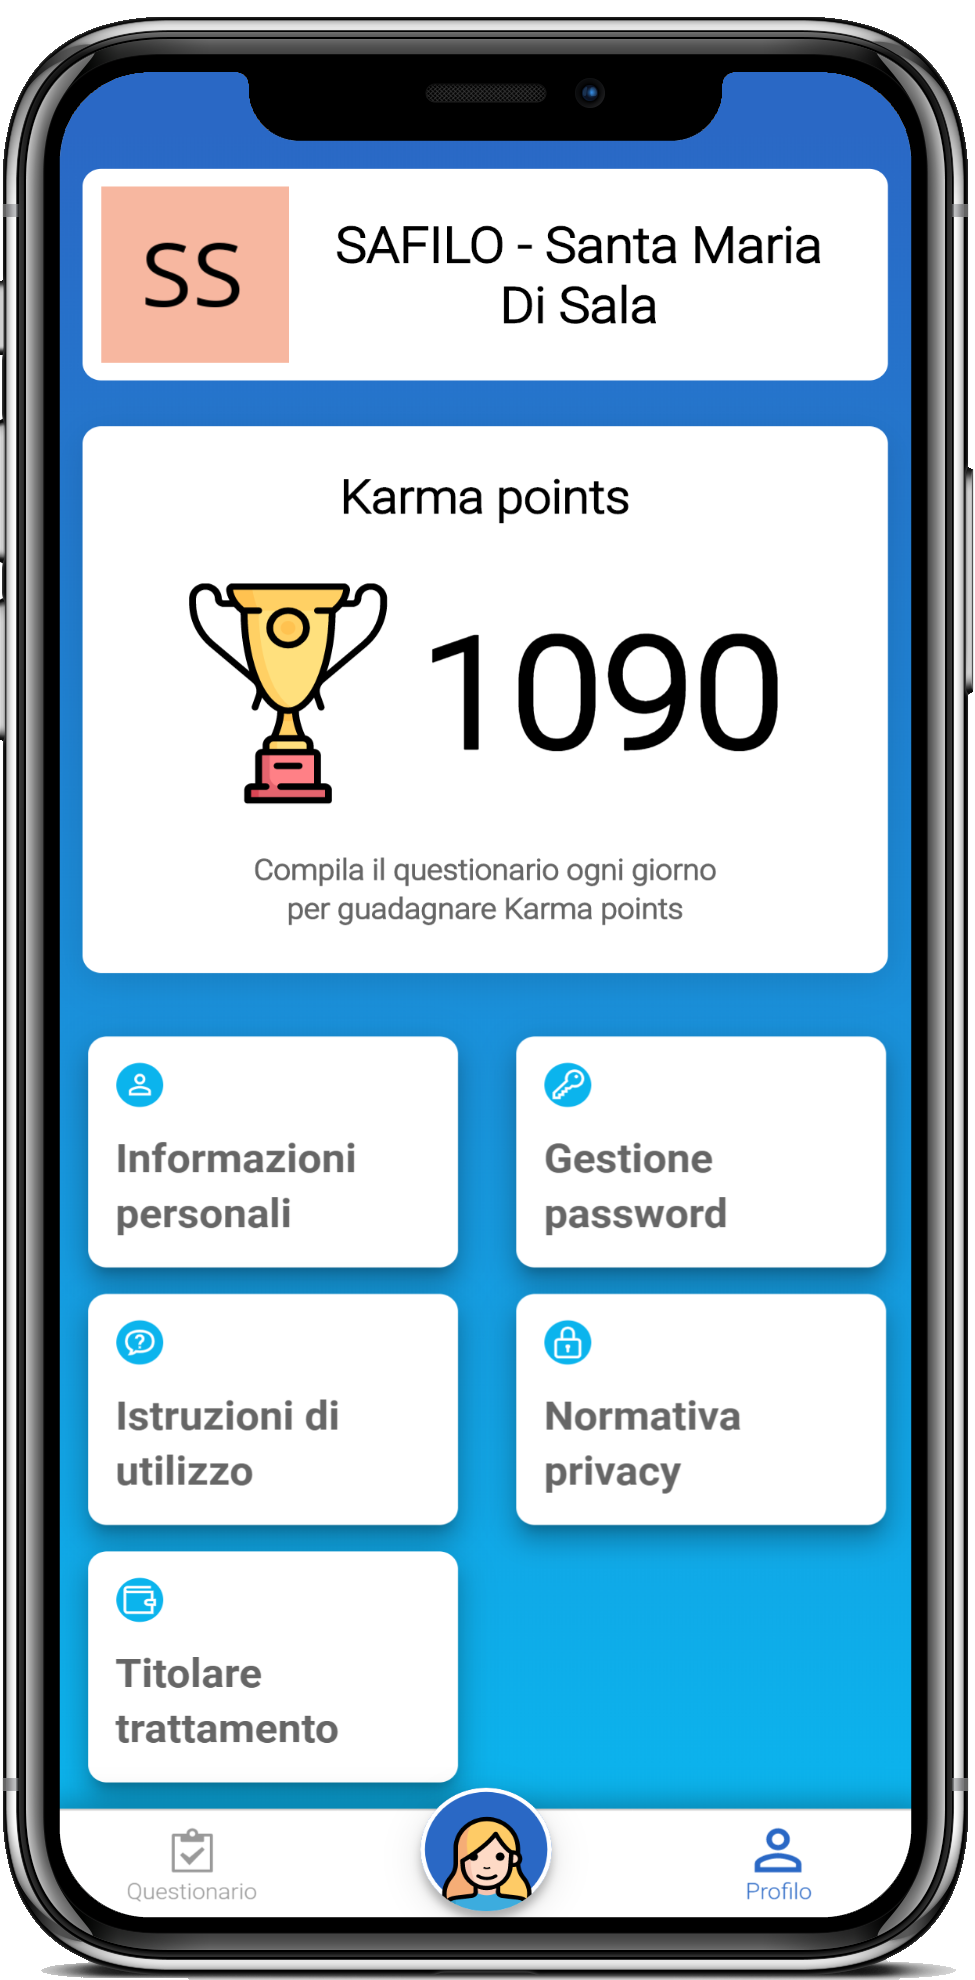
\includegraphics[scale=0.14]{profile.png}\hfil
			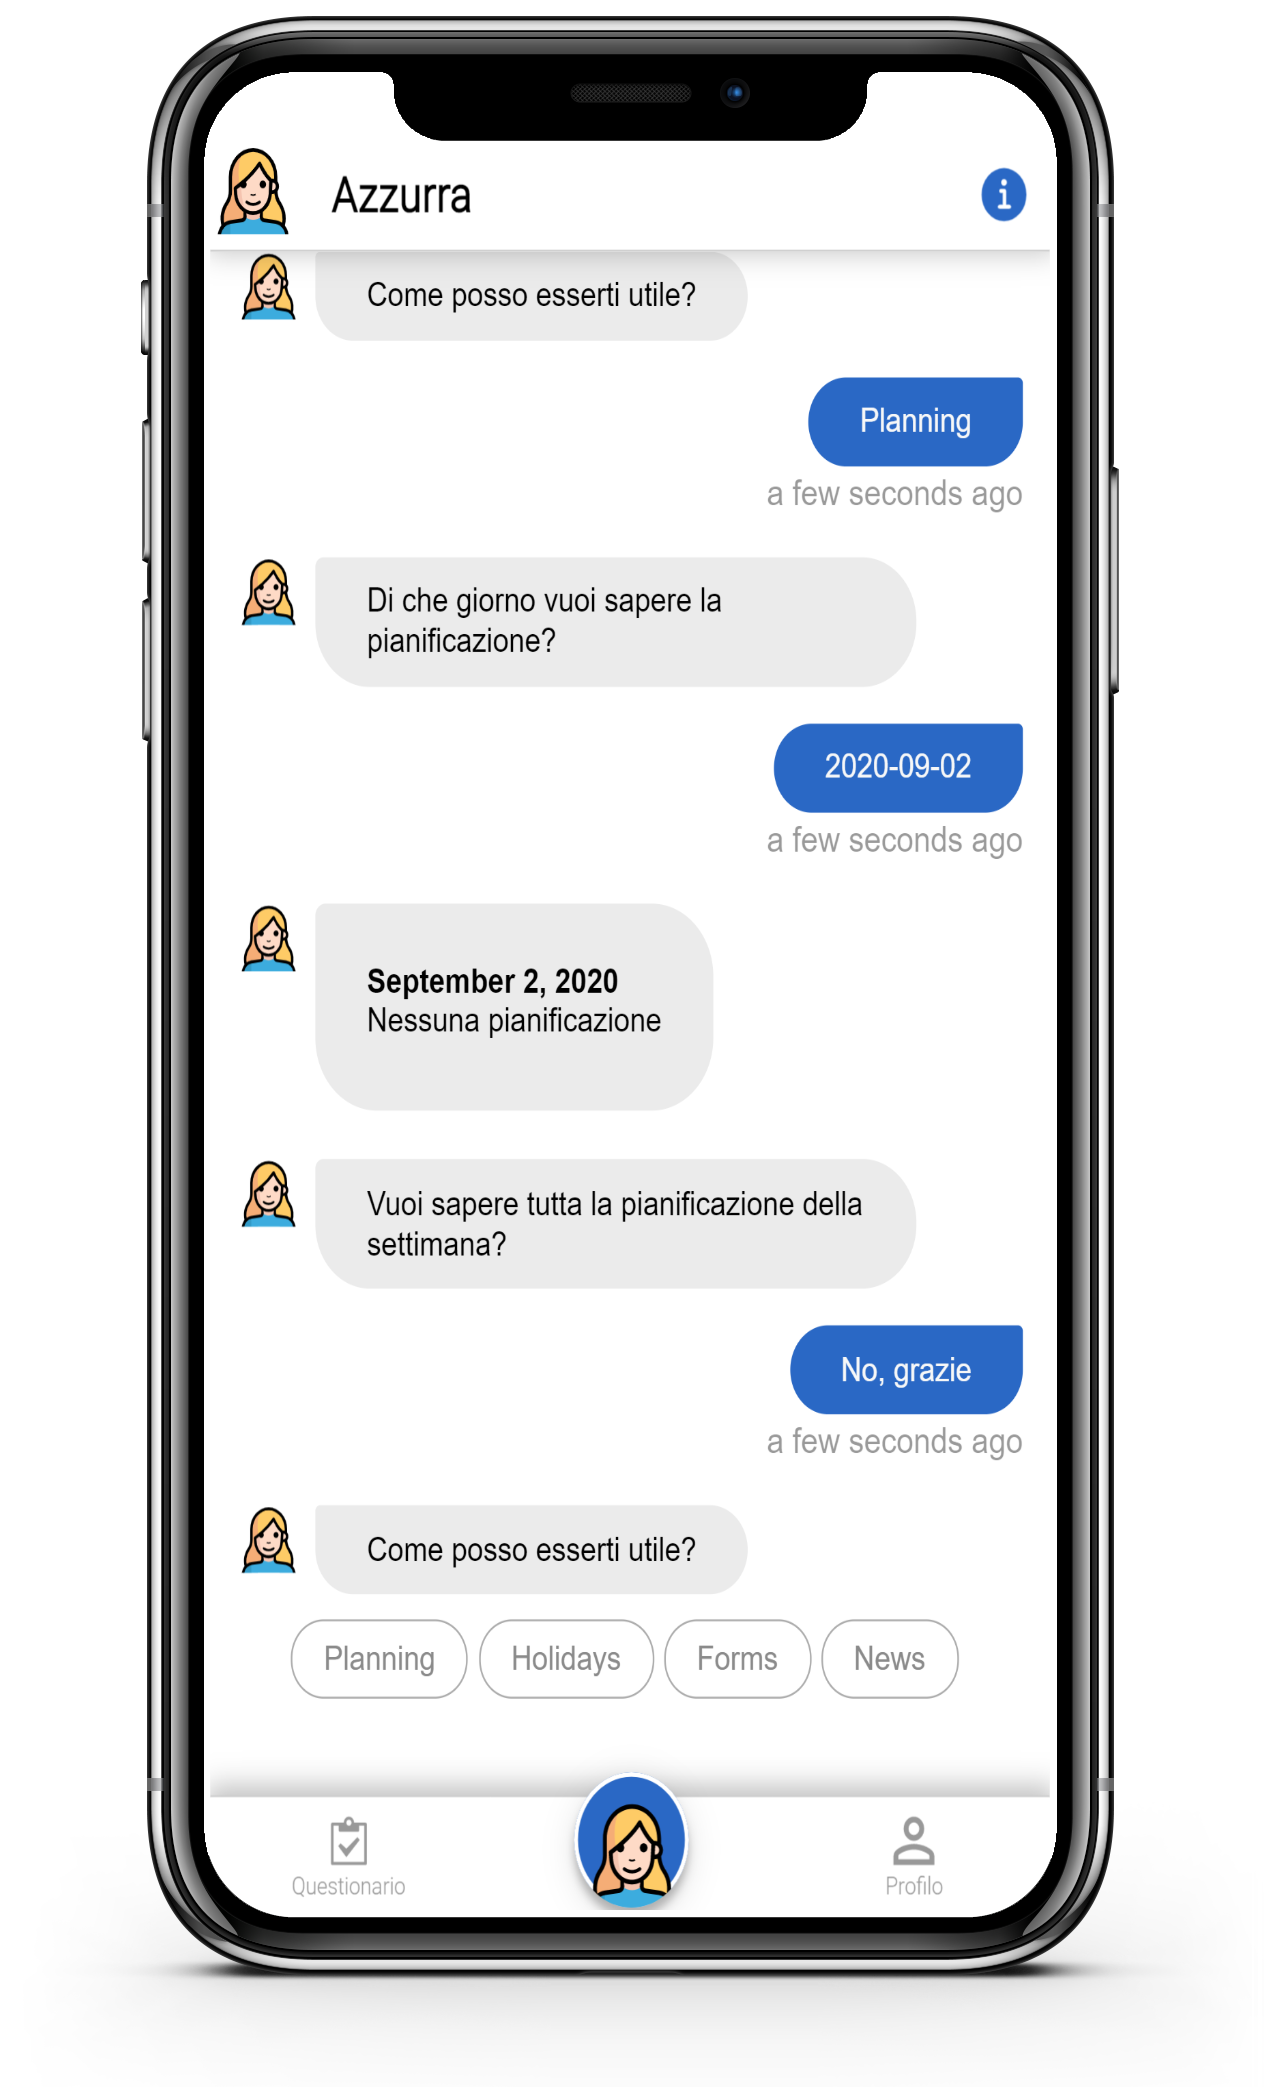
\includegraphics[scale=0.14]{chatAzzurra.png}
			\caption{Sezione Profilo e Chat con Azzurra}\label{fig:profile}
		\end{center}
	\end{figure}\\
	Nella sezione Azzurra, è presente la \emph{chat} \gls{bot}\ap{[g]} con Azzurra che attraverso il proprio flow engine, riesce a comprendere i flussi conversazionali ricevuti in input da Azzurra.io. Grazie a ciò il \gls{bot}\ap{[g]} Azzurra sa quali risposte e domande fare all'utente umano. Nel capitolo successivo verrà spiegato in modo dettagliato il funzionamento del Flow engine di Azzurra. Come detto precedentemente la comunicazione con Azzurra avviene attraverso \gls{WebSocket}\ap{[g]} che permette di tenere aggiornati i flussi conversazionali ricevuti da Azzurra nel caso in cui subiscano modifiche. Come scritto in precedenza, Azzurra è un \gls{bot}\ap{[g]} che aiuta il lavoratore a poter::
	\begin{itemize}
		\item Visualizzare il proprio turno di lavoro;
		\item Visualizzare i propri permessi lavorativi o richiederne di nuovi;
		\item Visualizzare avvisi da parte dell'azienda;
		\item Sapere qual'è il menu del giorno della mensa aziendale;
		\item Poter effettuare prenotazioni di un posto a sedere in una sala riunioni e visualizzare le proprie prenotazioni, inoltre utilizzare un scannerizzatore \gls{QR code}\glsfirstoccur per riscattare il posto prenotato.
	\end{itemize}
\end{trivlist}	
\subsubsection{Gestione modalità offline}	
Nell'ambito dello sviluppo di un'applicazione \emph{mobile}, un aspetto importante è la gestione della modalità \emph{offline}. Per gestione della modalità \emph{offline} si intende permette agli utenti di continuare ad utilizzare l'applicazione in assenza di connettività e quindi l'impossibilità di comunicare con il back-end. Quali e quante funzionalità e con quali e quante limitazioni alle stesse si verificano quando si è \emph{offline}, è una scelta di progettazione e comporta uno sforzo più o meno significativo visto che esistono diverse modalità per ottenere quanto richiesto. Nel caso dell'applicazione \emph{mobile} \gls{AWMS} in assenza di connettività sono state scelte le seguenti limitazioni e funzionalità:
\begin{itemize}
	\item Quando c'è assenza di connettività viene avvisato l'utente di tale evento, attraverso un messaggio che comparirà sopra l'\emph{header} dell'applicazione;
	\item Vengono garantite un insieme minimo di funzionalità anche in caso di assenza di connettività, nello specifico viene garantita all'utente la possibilità di spostarsi tra le sezioni dell'applicazione accedendo solo ad alcune pagine informative quali la "Informazioni personali", la "Privacy policy", le "Istruzioni di utilizzo" dell'applicazione.
\end{itemize}

La gestione della modalità \emph{offline} verterà principalmente su due aspetti:
\begin{itemize}
	\item stato della connessione;
	\item persistenza locale dei dati.
\end{itemize}
\subsubsection{Stato della connessione}
Poter sapere lo stato della connessione per il funzionamento dell'applicazione \emph{mobile} è fondamentale. Inoltre, è importante tenere conto che la connettività nel tempo cambia infatti, può accadere che l'utente sia connesso all'inizio ma ad un certo punto perde la connessione. Vi è quindi la necessità non solo di sapere lo stato della connessione all'inizio ma anche i cambiamenti nello stato della connettività. Solitamente per determinare lo stato della connessione si accede direttamente sullo strato nativo del \emph{device}. Per fare ciò è stato scelto di utilizzare il plugin di Cordova, Network Information, che oltre a determinare lo stato della connessione, è in grado di rilevare cambiamenti dello stato in maniera agevole.

\subsubsection{Persistenza locale dei dati}
Il poter salvare dei dati in locale offre la possibilità di poter garantire l'esecuzioni di alcune funzioni anche in assenza di connettività. Esistono diverse possibilità per la memorizzazione locale dei dati, più o meno sicure, più o meno efficienti.\\

Per l'applicazione \emph{mobile} \gls{AWMS} è stato scelto di utilizzare SQLite. SQLite è un \gls{DBMS}\ap{[g]} file-based memorizzato sul \emph{device} sul quale viene installata l'applicazione. La capacità del database (dimensione massima) dipende dalla memoria a disposizione nel \emph{device} offrendo quindi un buon supporto per la memorizzazione e l'esecuzione delle comuni operazioni sui dati.\\

L'applicazione \emph{mobile} essendo una \gls{applicazione ibrida}\ap{[g]} costruita con Ionic, è stato scelto di utilizzare Ionic Storage che si compone di un plugin di Cordova, per la gestione dei database SQLite.\\

Utilizzando Ionic Storage è possibile quindi memorizzare delle coppie chiave-valore dove il valore può essere di qualsiasi tipo,
dalle semplici stringhe o interi fino a degli oggetti \gls{JSON}\ap{[g]}. I dati memorizzati localmente rimarranno disponibili sino alla disinstallazione dell'applicazione o alla formattazione del \emph{device}.


\section{Operazioni}
Nella seguente sezione verranno descritte le principali operazioni tra le varie componenti dell'\gls{architettura}\ap{[g]}.
\subsection{Creazione di una connessione attreverso WebSocket}
Come spiegato in precedenza, la comunicazione tra l'applicazione \emph{mobile} e Azzurra.io avviene attraverso l'utilizzo di \gls{WebSocket}\ap{[g]}. Grazie a ciò si ha un canale di comunicazione a due vie cioè, sia l'applicazione \emph{mobile} e sia Azzurra.io possono inviare dati o richieste. Inoltre, le modifiche ai flussi conversazionali già esistenti o l'aggiunta di nuovi flussi, verranno comunicate all'applicazione \emph{mobile} in tempo reale, aggiornando perciò i dati posseduti dell'applicazione. Infine, utilizzando una connessione tramite \gls{WebSocket}\ap{[g]}, risulta essere più efficiente e performante rispetto al \gls{pooling}\glsfirstoccur perché il \gls{server}\ap{[g]} non viene continuamente contatto da inutili richieste.
\begin{figure}[h]
	\begin{center}
		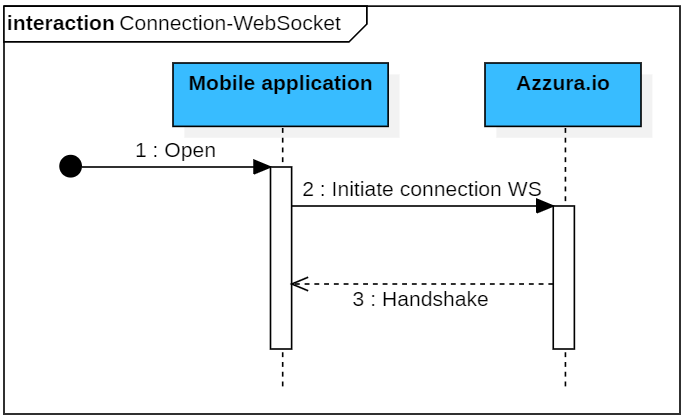
\includegraphics[scale=0.8]{Connection-WebSocket.PNG}
		\caption{Sequence diagram per la creazione di una connessione attraverso WebSocket}\label{fig:websocket}
	\end{center}
\end{figure}

Nella Figura~\ref{fig:websocket} viene mostrato come avviene la creazione di una connessione tra l'applicazione \emph{mobile} e Azzurra.io, i passi perciò sono:
\begin{enumerate}
	\item All'inizio, l'applicazione \emph{mobile} viene aperta dall'utente, essa cercherà da subito di mettersi in contatto con Azzurra.io creando una connessione;
	\item Per avviare una connessione \gls{WebSocket}\ap{[g]}, viene inviata una richiesta \gls{http}\ap{[g]} a Azzurra.io(\gls{server}\ap{[g]}). Tale richiesta \gls{http}\ap{[g]} HTTP ha la particolarità che negli \emph{headers} dell’intestazione viene specificata un'operazione di tipo \emph{Upgrade} cioè indica che l'applicazione \emph{mobile} (\gls{client}\ap{[g]}) vuole aggiornare la connessione ad un protocollo diverso, in questo caso a \gls{WebSocket}\ap{[g]}. Questo tipo di operazione prende il nome di \emph{WebSocket handshake request}.\\ \\
	\begin{lstlisting}
GET /mychat HTTP/1.1
Host: server.AzzurraIo.com
Upgrade: websocket	
Connection: Upgrade		
Sec-WebSocket-Key: 32ndfsMjnQiZXBijAfOiPni==
Sec-WebSocket-Protocol: chat		
Sec-WebSocket-Version: 13		
Origin: http://AzzurraIo.com
	\end{lstlisting}
	Il codice soprastante rappresenta un esempio di \emph{WebSocket handshake request} inviata dal \gls{client}\ap{[g]} al \gls{server}\ap{[g]}. Il \gls{client}\ap{[g]} inserisce una stringa casuale codifica in \gls{base64}\ap{[g]} nel campo \emph{Sec-WebSocket-Key} alla quelle viene poi aggiunta una stringa fissa.
	\item Se il \gls{server}\ap{[g]}, in questo caso Azzurra.io supporta la connessione tramite \gls{WebSocket}\ap{[g]} allora rispondere mettendo nel campo \emph{Sec-WebSocket-Accept} la risposta cioè, l'hash della stringa contenuta in \emph{Sec-WebSocket-Key} utilizzando la funzione di hashing SHA-1. Infine, viene tutto codificato in \gls{base64}\ap{[g]}. Una volta arrivata la risposta al \gls{client}\ap{[g]}, esso controllerà se la risposta contiene la stringa corretta. Tutte queste operazioni hanno lo scopo di evitare di aprire più connessioni multiple ma non da nessuna garanzia di autenticazione.
	Nel seguente codice viene riportato un esempio di risposta da parte del server.\\
	\begin{lstlisting}
HTTP/1.1 101 Switching Protocols
Upgrade: websocket
Connection: Upgrade
Sec-WebSocket-Accept: fPmrc0slUIUYIuyY2HaGWk=
Sec-WebSocket-Protocol: chat
	\end{lstlisting}
\end{enumerate}
Per garantire una comunicazione sicura contro ascoltatori terzi viene usata una variante del \gls{WebSocket}\ap{[g]} detta \emph{Secure WebSocket (WSS)} che utilizza il protocollo HTTPS al posto del protocollo \gls{http}\ap{[g]}
\subsection{Recupero di un flusso conversazionale}
\begin{figure}[h]
	\begin{center}
		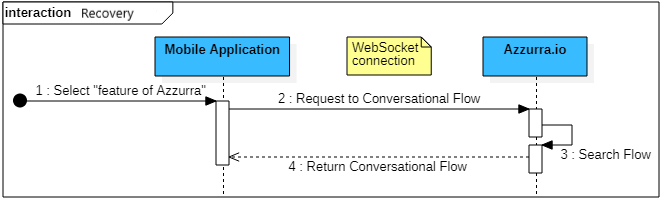
\includegraphics[scale=0.75]{recovery.png}
		\caption{Sequence diagram per il recupero di un flusso conversazionale}\label{fig:recovery}
	\end{center}
\end{figure}
Il \gls{bot}\ap{[g]} Azzurra per poter funzionare ha bisogno di almeno un flusso conversazionale che grazie alla propria struttura, permette al flow engine di Azzurra di comprendere il flusso e capire quali messaggi deve far visualizzare ad Azzurra nella \emph{chat} con l'utente umano. I flussi si trovano nel database dedicato di Azzurra.io. Quando viene richiesto di fare un’operazione o si inizia per la prima volta un'interazione con Azzurra, essa per sapere cosa fare ha bisogno di uno specifico flusso di conversazione, nel caso in cui sia la prima interazione con l'utente, richiedere il cosiddetto \emph{MainFlow} dove vengono riportate quali funzionalità Azzurra può offrire. Se invece si è nel caso in cui l'utente richiede una specifica funzionalità ad esempio richiedere la visualizzazione del piano di lavoro, Azzurra dovrà richiedere a Azzurra.io, il \emph{flow} dedicato alla specifica funzionalità.
Come mostrato nella Figura~\ref{fig:recovery} si hanno i seguenti passi:
\begin{enumerate}
\item L'utente interagisce con il \gls{bot}\ap{[g]} Azzurra e richiede una funzionalità oppure l'utente interagisce con Azzurra per la prima volta;
\item Il \gls{bot}\ap{[g]} Azzurra tramite una connessione aperta precedentemente chiede a Azzurra.io il corretto \emph{flow} per poter soddisfare le richieste dell'utente. Si sottolinea che ogni \emph{flow} ha un codice identificativo che lo identifica e Azzurra sa sempre qual'è il codice identificativo del flusso di cui ha bisogno;
\item Azzurra.io cerca nel proprio database se contiene il \emph{flow} richiesto;
\item Se la ricerca da esito positivo allora Azzurra.io ritornerà il flusso che verrà eseguito dal flow engine di Azzurra la quale proseguirà con la conversazione. Se invece non lo trova la conversazione si interrompe mostrando nella \emph{chat} un messaggio di errore.
\end{enumerate}

\subsection{Richiesta e invio di dati}
Durante l'esecuzione di una conversazione è molto probabile che Azzurra abbia bisogno di far visualizzare delle informazioni richieste dall'utente ad esempio il suo orario di lavoro, queste informazioni però non sono salvate ne nell'applicazione mobile né in Azzurra.io ma nel back-end.
\begin{figure}[h]
	\begin{center}
		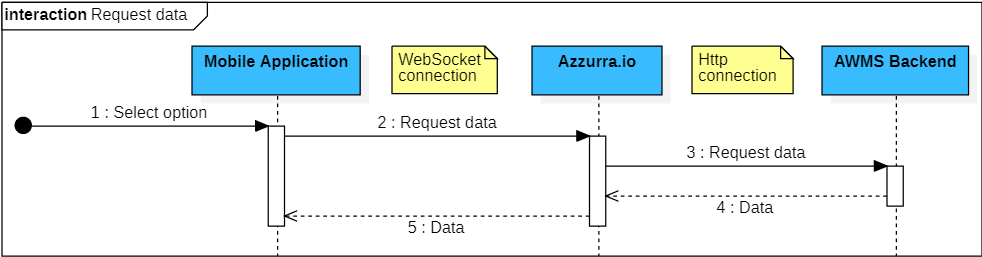
\includegraphics[height=5cm, width=13cm]{request.png}
		\caption{Sequence diagram per il recupero dei dati sul lavoratore}\label{fig:request}
	\end{center}
\end{figure}
La Figura~\ref{fig:request} mostra come Azzurra ottiene i dati richiesti:
\begin{enumerate}
	\item L'utente chiede una qualche operazione ad Azzurra che necessita contattare il back-end per ottenere i dati che l'utente vuole;
	\item L'applicazione chiede quindi i dati necessari a Azzurra.io che si prende carico della richiesta;
	\item Azzurra.io contatta il back-end attraverso una richiesta \gls{http}\ap{[g]}, per richiedere i dati richiesti da Azzurra;
	\item Se la richiesta va a buon fine il back-end ritornerà i dati ad Azzurra.io che li ritornerà a sua volta ad Azzurra.
\end{enumerate}
Per l'invio dei dati cioè l'utente inserisce dei dati che devono essere salvati sul database del backend, ad esempio l'utente inserisce una nuova assenza, il procedimento sarà analogo alla richiesta di dati solo alla fine non verranno ritornati i dati ma l'esito dell'operazione effettuata.
\subsection{Gestione notifiche push}
Nel caso in cui il \gls{plant manager}\ap{[g]} abbia bisogno di mandare una comunicazione a uno o più lavoratori, è stata implementata la possibilità di inviare delle notifiche contenti la comunicazione.
\begin{figure}[h]
	\begin{center}
		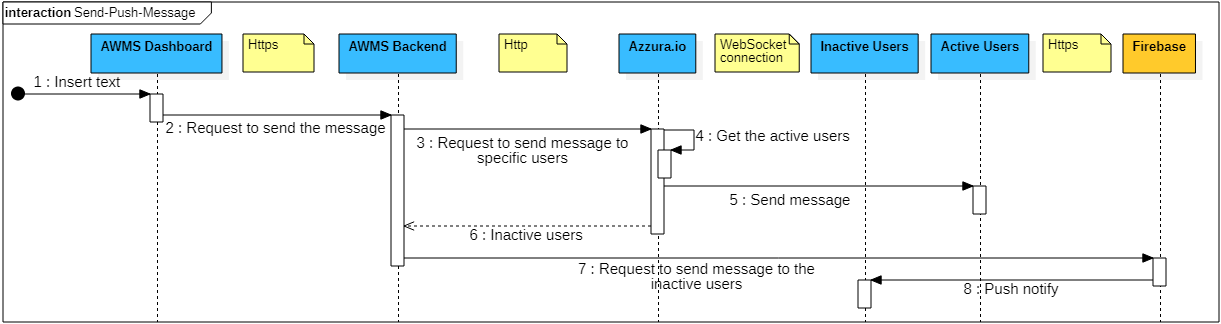
\includegraphics[height=6cm, width=14cm]{pushMex.png}
		\caption{Sequence diagram per l'invio di notifiche push}\label{fig:push}
	\end{center}
\end{figure}\\
Nella Figura~\ref{fig:push} viene mostrato come avviene l'invio delle notifiche, di seguito ne vengono descritti i passi:
\begin{enumerate}
	\item Il \gls{plant manager}\ap{[g]} crea il messaggio da inviare attraverso l'interazione con la dashboard di \gls{AWMS};
	\item La \emph{dashboard} invia al back-end il messaggio da inviare e a quali utenti registrati nel sistema mandare il messaggio, viene perciò mandato oltre al messaggio anche i codici identificativi dei destinatari;
	\item Il back-end si connette ad Azzurra.io e gli invia il messaggio e la lista degli utenti a cui deve mandare la notifica. Quindi l'invio della notifica viene delegato a Azzurra.io; 
	\item Azzurra.io controlla sulla sua tabella \emph{User Map}, quali tra gli utenti che devo ricevere il messaggio sono attualmente connessi al \emph{socket}. Si specifica inoltre che vengono considerati utenti connessi o attivi tutti gli utenti che sono connessi al \emph{socket} e che hanno l’applicazione in \gls{foreground}\ap{[g]}. Gli utenti che sono connessi al \emph{socket}, ma hanno l’applicazione in \gls{background}\ap{[g]} vengono trattati come utenti non connessi;
	\item Per gli utenti connessi al \emph{socket}, Azzurra.io invierà la notifica ai dispositivi connessi in cui verrà visualizzata sotto forma di messaggio da parte di Azzurra;
	\item Nel caso in cui ci siano alcuni utenti non connessi a Azzurra.io tra i destinatari del messaggio, Azzurra.io effettua una richiesta \gls{http}\ap{[g]} ad AWMS Backend, specificando gli utenti che non è riuscita a contattare, e il messaggio che avrebbe dovuto recapitare;
	\item Il back-end una volta ricevuta la lista degli utenti a cui non è stato possibile mandare la notifica, contatterà attraverso un \gls{api}\ap{[g]} di Firebase, quest'ultimo per richiedere l'invio della notifica agli utenti della lista appena ricevuta. Si specifica che Firebase sarà in grado di farlo solo se i dispositivi dei destinatari si sono sottoscritti al servizio di Firebase per la ricezione di una \gls{notifica push}\ap{[g]};
	\item Firebase ricevuta la lista d'utenti a cui inviare la notifica e il testo del messaggio, invierà la \gls{notifica push}\ap{[g]} ai destinatari.
\end{enumerate}